% PLEASE USE THIS FILE AS A TEMPLATE
% Check file iosart2x.tex for more examples

% add. options: [seceqn,secthm,crcready,onecolumn]
\documentclass[sw]{iosart2x}

%\usepackage{dcolumn}
%\usepackage{endnotes}

\usepackage{url}
\usepackage{todonotes}
\usepackage{booktabs}
\usepackage{pgfplots}
\usepackage{aurl}
\usepackage{upgreek}
\usepackage{subfigure}
\usepackage{amsfonts}
\usepackage{amssymb}
\usepackage{amsmath}
\usepackage{graphicx}
\usepackage{tabularx}
%\usepackage{algorithmicx}
\usepackage{algorithm}
\usepackage{algpseudocode}
\usepackage{hyperref}
\usepackage{multicol}
%tr: used for strikeout in comments
\usepackage[normalem]{ulem}

\usepackage[utf8]{inputenc}
\usepackage[T1]{fontenc}
\usepackage[scaled=0.85]{beramono}
\usepackage{listings}
\usepackage{filecontents}
\usepackage{float}
\usepackage{todonotes}
\lstset{language=SQL,morekeywords={PREFIX,java,rdf,rdfs,url}}
\usepackage{pifont}% http://ctan.org/pkg/pifont
\usepackage{xcolor}
\usepackage{mdframed}
\usepackage{siunitx}
\DeclareSIUnit{\nothing}{\relax}
\usepackage{listings}
\usepackage{csquotes}
\usepackage{colortbl}


%New colors defined below
\definecolor{codegreen}{rgb}{0,0.6,0}
\definecolor{codegray}{rgb}{0.5,0.5,0.5}
\definecolor{codepurple}{rgb}{0.58,0,0.82}
\definecolor{backcolour}{rgb}{0.95,0.95,0.92}

%Code listing style named "mystyle"
\lstdefinestyle{mystyle}{
  backgroundcolor=\color{backcolour},   commentstyle=\color{codegreen},
  keywordstyle=\color{magenta},
  numberstyle=\tiny\color{codegray},
  stringstyle=\color{codepurple},
  basicstyle=\ttfamily\footnotesize,
  breakatwhitespace=false,         
  breaklines=true,                 
  captionpos=b,                    
  keepspaces=true,                 
  numbers=left,                    
  numbersep=5pt,                  
  showspaces=false,                
  showstringspaces=false,
  showtabs=false,                  
  tabsize=2
}

%"mystyle" code listing set
\lstset{style=mystyle}

\usepgfplotslibrary{groupplots}
\usetikzlibrary{patterns}

\newcommand{\xmark}{\ding{55}}%
\usetikzlibrary{graphs}

\newcommand{\E}{{\mathcal{E}}}
\newcommand{\F}{{\mathcal{F}}}
\newcommand{\ds}{{\ensuremath{D_s}}}
\newcommand{\dt}{{\ensuremath{D_t}}}

\newcommand{\func}[2]{\textnormal{#1}(#2)}
\newcommand{\f}[1]{\func{f}{#1}}
\newcommand{\h}[1]{\func{h}{#1}}
\newcommand{\saleem}[1] {\textcolor{blue}{[saleem]\textit{#1}}}

\usepackage[capitalise,nameinlink]{cleveref}
%Nice formats for \cref                                                                                  
\crefname{section}{Section}{Section}
\crefname{table}{Table}{Table}
\Crefname{section}{Section}{Sections}
\crefname{figure}{Fig.}{Fig.}
\Crefname{figure}{Figure}{Figures}


\pubyear{2020}
\volume{0}
\firstpage{1}
\lastpage{1}

\begin{document}

\begin{frontmatter}

%\pretitle{}
\title{Identifying, Querying, and Relating Large Heterogeneous RDF Sources}
\runningtitle{Identifying, Querying, and Relating Large Heterogeneous RDF Sources}
%\subtitle{}

% \author{Andre Valdestilhas\inst{1} \and Tommaso Soru\inst{1} \and Muhammad Saleem\inst{1} \and Edgard Luiz Marx\inst{2} \and Wouter Beek \and Claus Stadler\inst{1} \and Thomas Riechert\inst{2} \and Oscar Corcho\inst{3}}

% \institute{
% AKSW Group\\ University of Leipzig, Germany\\
% \email{\{valdestilhas,tsoru,saleem,cstadler\}@informatik.uni-leipzig.de}
% \\Leipzig University of Applied Science (HTWK)\\
% \email{\{marx,thomas.riechert\}@htwk-leipzig.de}
% \\Ontology Engineering Group. Universidad Politecnica de Madrid. Boadilla del Monte, Spain\\
% \email{ocorcho@fi.upm.es}
% }
\author[A]{\fnms{Andre} \snm{Valdestilhas}}
\author[A]{\fnms{Tommaso} \snm{Soru}}
\author[A]{\fnms{Muhammad} \snm{Saleem}}
\author[B]{\fnms{Edgard} \snm{Marx}}
\author[C]{\fnms{Wouter} \snm{Beek}}
\author[A]{\fnms{Claus} \snm{Stadler}}
\author[D]{\fnms{Bernardo} \snm{Pereira Nunes}}
\author[E]{\fnms{Konrad} \snm{Höffner}}
\author[B]{\fnms{Thomas} \snm{Riechert}}

\address[A]{
  Computer Science Institute, University of Leipzig,
  \href{mailto:valdestilhas@informatik.uni-leipzig.de, mailto:tsoru@informatik.uni-leipzig.de, mailto:saleem@informatik.uni-leipzig.de, mailto:cstadler@informatik.uni-leipzig.de}{\{valdestilhas,tsoru,saleem,cstadler\}@informatik.uni-leipzig.de}
}

\address[B]{
  Leipzig University of Applied Science (HTWK),
  \href{mailto:edgard.marx@htwk-leipzig.de, mailto:thomas.riechert@htwk-leipzig.de}{\{edgard.marx, thomas.riechert\}@htwk-leipzig.de}
}

\address[C]{
VU University Amsterdam (VUA)
\href{mailto:w.g.j.beek@vu.nl}{w.g.j.beek@vu.nl}
}

\address[D]{
  Australian National University (ANU),
  \href{mailto:bernardo.nunes@anu.edu.au}{bernardo.nunes@anu.edu.au}
}

\address[E]{
  Institute for Medical Informatics, Statistics and Epidemiology (IMISE),
  \href{mailto:konrad.hoeffner@imise.uni-leipzig.de}{konrad.hoeffner@imise.uni-leipzig.de}
}

% \todo[inline]{ED: You have to standardize the graphs, every graph seems different style, size and formatting than the other}

%\todo[inline]{ED: Try to solve all latex compilation problems. KH: I took care of all the compilation errors. Mostly it was due to unescaped underscores in the DOIs in the .bib files. P.S.: Nathanel says we can fix this also by switching to biblatex}

% \todo[inline]{ED: Fig 1, 2 and 3 should be redesigned}

% \todo[inline]{ED: Fig 5. is very hard to understand, better add one graph for each dataset separately and instead of calling D1... call it by the name e.g. DBpedia, Wikidata }

% \todo[inline]{ED: Fig 6. you should remove the text from the Figure and add it bellow in the Captions.}

% \todo[inline]{ED: Fig 7. this figure should use the same style as Fig 6 Pie charts.}

% \todo[inline]{ED: I could not find the similarity Table that I  asked you? It should encode information like this one here \url{http://www.scielo.br/img/revistas/gmb/v27n1/a14tab03.gif}}

\runningauthor{Valdestilhas et al.}

% \author[A]{\inits{N.}\fnms{Name1} \snm{Surname1}\ead[label=e1]{first@somewhere.com}%
% \thanks{Corresponding author. \printead{e1}.}},
% \author[B]{\inits{N.N.}\fnms{Name2 Name2} \snm{Surname2}\ead[label=e2]{second@somewhere.com}}
% and
% \author[B]{\inits{N.-N.}\fnms{Name3-Name3} \snm{Surname3}\ead[label=e3]{third@somewhere.com}}
% \runningauthor{N. Surname1 et al.}
% \address[A]{Department first, \orgname{University or Company name},
% Abbreviate US states, \cny{Country}\printead[presep={\\}]{e1}}
% \address[B]{Department first, \orgname{University or Company name},
% Abbreviate US states, \cny{Country}\printead[presep={\\}]{e2,e3}}

%\begin{review}{editor}
%\reviewer{\fnms{First} \snm{Editor}\address{\orgname{University or Company name}, \cny{Country}}}
%\reviewer{\fnms{Second} \snm{Editor}\address{\orgname{First University or Company name}, \cny{Country}
%    and \orgname{Second University or Company name}, \cny{Country}}}
%\end{review}
%\begin{review}{solicited}
%\reviewer{\fnms{First} \snm{Solicited reviewer}\address{\orgname{University or Company name}, \cny{Country}}}
%\reviewer{\snm{anonymous reviewer}}
%\end{review}
%\begin{review}{open}
%\reviewer{\fnms{First} \snm{Open Reviewer}\address{\orgname{University or Company name}, \cny{Country}}}
%\end{review}

\begin{abstract}
Although we have witnessed a growing adoption of Linked Open Data principles for publishing data on the Web, connecting data to third parties remains a difficult and time-consuming task. One question that often raises during the publication process is: ``Is there any data set available on the Web we can connect with?". This simple question unfolds a set of others that hinders data publishers to connect to other data sources. For instance, if there are related data sets, where are they? How many? Do they share concepts and properties? How similar are they? Is there any duplicated data set? How to identify and query a huge amount of heterogeneous datasets.
To answer these questions, this paper introduces: (i) a new class of data repositories; (ii) a method to identify datasets containing a given URI; (iii) a query engine and source selection in a large RDF dataset collection; (iv) a novel method to detect and store data set similarities including duplicated data set and data set chunk detection; (v) an index to store data set relatedness; and, (vi) a search engine to find related data sets.
To create the index, we harvested more than \SI{668}{\kilo\nothing} data sets from LOD Stats and LOD Laundromat, along with 559 active SPARQL endpoints corresponding to 221.7 billion triples or 5 terabytes of data. 
Our evaluation on state-of-the-art real-data shows that more than 90\% of data sets in the LOD Laundromat do not use \textit{owl:equivalentProperty} or \textit{owl:equivalentClass} to relate to one another data, which reaffirms and emphasizes the importance of our work.
\end{abstract}

\begin{keyword}
\kwd{Indexing}
\kwd{Querying the Web of Data}
\kwd{Federated Query}
\kwd{Source selection}
\kwd{Big Data techniques}
\kwd{Integrating different sources}
\kwd{Identifying datasets}
\end{keyword}

\end{frontmatter}

\section{Introduction}
% Move 1 - Establishing a research territory (introducing and reviewing items of previous research in this area)

Due to the heterogeneity of the datasets, this uniqueness is reflected in the datasets structure, making it a hard task to find relations among those datasets, i.e. to identify how similar they are.
In this way, we can say that Linked Data involves datasets and linksets and those linksets needs to be maintained.
There are many ways to maintain linksets, one of those is to create a semantic web link repository, e.g. LinkLion \cite{linklion2014}.

% Move 2 - Establishing a niche (highlighting gap; by indicating a gap in previous research or by extending previous knowledge in some way)
% Move 3 - Occupying the niche (previewing new accomplishments; outlining purposes or stating the nature of the present research, research question or hypotheses, stating value)

The concept of Linked Data relates to a collection of best practices to publish and connect structured web-based data.
However, the number of available datasets has been growing significantly over the last decades \cite{bizer2011linked}.
Those datasets represent now the well known as Web of Data, which represents a large collection of concise and detailed interlinked data sets from multiple domains with large datasets \cite{saleem2013linked}.
Thus, linking entries across heterogeneous data sources, such as databases or knowledge bases, becomes an increasingly difficult issue \cite{valdestilhas2017high, NGAU11, saeedi2018scalable}.
However, connections between datasets play a leading role in significant activities such as cross-ontology question answering \cite{lopez2009cross}, large-scale inferences \cite{urbani2010owl} and data integration \cite{rahm2016case}.
In Linked Data, the linksets are well known for executing the task of generating links between datasets \cite{NGAU11}.

The current challenges addressed in this paper are identifying and querying datasets from a huge heterogeneous collection of RDF datasets.
In order to execute these tasks, we need to know how the datasets are related and how similar they are.
We present and discuss the need to identify and query the relation of those datasets.

To deal with the need for identifying LOD Datasets, we created called "Where is my URI?"(WIMU)~\cite{valdestilhas2018my} a regularly updated database index of more than \SI{660}{\kilo\nothing} datasets from LODStats and LOD Laundromat, an efficient, low cost and scalable service on the web that shows, which dataset most likely defines a URI and various statistics of datasets indexed from LODStats and LOD Laundromat.
In \cite{valdestilhas2019more} we show how to integrate and querying LOD datasets, we provide a hybrid SPARQL query processing engine that is able to retrieve results from 559 active SPARQL endpoints (with a total of 163.23 billion triples) and \num{668166} datasets (with a total of 58.49 billion triples) from LOD Stats and LOD Laudromat.
In this paper we will show an extention of those works\cite{valdestilhas2018my, valdestilhas2019more} showing how the datasets are related and how similar they are.
To this aim we provide the LOD Dataset Relation Index called ReLOD, which provides information about how similar all the datasets from the LOD cloud are.%, including statistics about the current state of those datasets.

%improvements on semantic web link repositories related to how the datasets are related and how similar they are, Identifying and querying those datasets.

\subsection{The need for identifying and querying LOD datasets}
%\todo[inline]{WIMU and wimuQ.}
One of the Semantic Web foundations is the possibility to dereference URIs to let applications negotiate their semantic content.
However, this exploitation is often infeasible as the availability of such information depends on the reliability of networks, services, and human factors.
Moreover, it has been shown that around 90\% of the information published as Linked Open Data is available as data dumps and more than 60\% of endpoints are offline\cite{hogan2016linked}.
To this end, there is a need for a service to \textit{identify}, in which dataset a URI is defined, in order to let Linked Data consumers find the respective RDF data source, in case such information cannot be retrieved from the URI alone.

In order to \textbf{query} such an amount of LOD datasets, various interfaces, such as LOD Stats \cite{auer2012lodstats}, LOD Laudromat \cite{beek2014lod}, and SPARQL endpoints provide access to the hundreds of thousands of RDF datasets, representing billions of facts.
These datasets are available in different formats such as raw data dumps, HDT files, or directly accessible via SPARQL endpoints.
Querying such a large amount of distributed data is particularly challenging and many of these datasets cannot be directly queried using the SPARQL query language. %To deal with such problems we present WIMU~\cite{valdestilhas2018my} and wimuQ\cite{ValdestilhasKcap}.

\subsection{The need for integration and relation of LOD datasets}

People will always describe knowledge in different ways, due to the individuality of the being, different points of view, time and space, in which we assume as a natural phenomenon and standard.
Aware of the state of the art from Ontology/Schema/Instance Matching from Linked Data from venues such as VLDB\footnote{\url{https://www.vldb.org/}}, OEAI\footnote{\url{http://oaei.ontologymatching.org/}}, ISWC\footnote{\url{https://iswc2019.semanticweb.org/}}, ESWC\footnote{\url{https://2019.eswc-conferences.org/}}, among others, we observe that the LOD datasets are following this standard.

We harvested more than \SI{668}{\kilo\nothing} data sets from LOD Stats and LOD Laundromat, along with 559 active SPARQL endpoints corresponding to 221.7 billion triples or 5 terabytes of data. We observed several duplicates and chunks among the datasets and the fact that more than 90\% of data sets in the LOD Laundromat do not use \textit{owl:equivalentProperty} or \textit{owl:equivalentClass}\footnote{Some concepts, such as skos:closeMatch, skos:exactMatch, and owl:sameAs were excluded from this study because they are not relevant enough to identify the equivalence of properties.} to relate to one another data, which reaffirms and emphasizes the importance of our work.

We notice that there are several similar data sets.
Yet, there is no place that stores or provides such kind of information about how similar the data sets are and which attributes the data sets share. This work aims to build an index to store the relation among the data sets to have a place to see how similar the data sets are. We provide a method to index the relations among LOD data sets\footnote{Data sets from LODStats, LODLaundromat, and endpoints} based on the properties and classes that they share.

%We start giving two examples about how useful the index can be:
As a motivation of our work, we describe two distinct scenarios where the proposed index may be useful:

\textbf{Scenario 1}(\textit{finding datasets}): Given the SPARQL query at \cref{lst:scenario1}, the user wants to know if a given data set contains three properties, in which the user already know the query performs well at the SPARQL endpoint from CKAN\footnote{  CKAN SPARQL endpoint~\url{https://linked.opendata.cz/sparql}}:

\begin{lstlisting}[language=SPARQL, label={lst:scenario1}, caption=Scenario 1.]
SELECT * WHERE { ?s ?p ?o.
FILTER(?s=<http://purl.org/dc/terms/date> || 
?s=<http://crime.rkbexplorer.com/id/location> || 
?s=<http://purl.org/dc/terms/subject>
)}
\end{lstlisting}

The following questions are raised:
\begin{itemize}
    \item How to know which data sets are able to execute the query?
    \item Which of the data sets contains the most valuable results?
    \item Could the results from different data sets complement each other?
\end{itemize}

In this case an approach is needed to enable the user to know more datasets to extract the required information. An index of dataset relations and similarities could be used to know that the query can also be executed with results at \url{https://eu.dbpedia.org/sparql} but not at \url{http://dbpedia.org/sparql}, and we can execute at least five\footnote{Datasets available here: \url{https://tinyurl.com/5dataset}} other data sets to complement the results.

\textbf{Scenario 2}(\textit{finding properties}): The user needs information about cities from all datasets in your repository, more specifically datasets that are compatible with the class \url{http://dbpedia.org/ontology/City}.
Using our previous approach WIMU~\cite{valdestilhas2018my}, this URI was found in 11 datasets\footnote{Datasets available here: \url{https://tinyurl.com/wimuDbpediaCity}}, but how many URIs in other datasets that also represents a city that were not listed, for instance a city at WikiData\footnote{\url{https://www.wikidata.org/}} is represented by  \url{https://www.wikidata.org/wiki/Property:P131}.
We consider here that to execute such task manually on more than \num{600000} datasets is not feasible.
Thus, having an index of dataset relation will help in this case.

\subsection{Compliance with Linked Data rules and LOD Cloud}
%\todo[inline]{tr: Better Compliance with \sout{the four} Linked Data rules and LOD Cloud}
Aware of the four rules on Linked Data\cite{designissues-linkeddata}, we justify our work concerning these rules.%\todo[inline]{kh: are you sure you need to include this? as far as I know, the semantic journal uses another 5 star scheme and requires it only for linked data set descriptions: \url{http://www.semantic-web-journal.net/content/five-stars-linked-data-vocabulary-use}. }
(1) \textit{Use URIs as names for things}, in which all the work presented here uses URIs as names for things, and WIMU~\cite{valdestilhas2018my} is the largest index to locate datasets containing a given URI.
(2) \textit{Use HTTP URIs so that people can look up those names}, where WIMU~\cite{valdestilhas2018my} is an index allowing people lookup datasets for a given URI. Facilitating people to look up those names. (3) \textit{When someone looks up a URI, provide useful information, using the standards (RDF*, SPARQL)}. Our approach, WimuQ\cite{valdestilhas2019more}, allows obtaining information from URIs non-dereferenceable anymore, providing more source of data, making an Intelligent Source Selection to achieve more results from a given SPARQL query. (4) \textit{Include links to other URIs, so that they can discover more things}. ReLOD, which is the extension of WIMU and WIMUQ, which has the aim of identifying similar datasets that share properties and classes, by using the WIMU lookup index, the user can lookup datasets from a given URI and by using WIMUQ to dereference URIs non-dereferenceable anymore. ReLOD allows for discovering more information by the similarity of the datasets, for a given input that can be a Dataset, Property, Class, or SPARQL query.

Concerning the LOD-cloud dataset, which currently contains \num{1239} datasets with \num{16147} links (as of March 2019)\cite{lodcloud}. There are more than \num{600000} datasets from LODLaundromat, LODStats, and public SPARQL endpoints. One of our intentions is to provide ways to build a new version of the LOD-cloud with all those more than \SI{600}{\kilo\nothing} datasets, to help this aim we provide an index containing the similarity level of the datasets. As a first step, we present the ReLOD, showing a methodology to store the similarity level of all datasets. The index is queryable, accepting as input the dataset, SPARQL query, properties and classes, and giving as output the respective similar datasets, properties, and classes.

%The contributions of this paper are:
To deal with all needs presented before we create an integrated approach to identify, relate and query a massive amount of heterogeneous RDF sources, in which join the two previous works\cite{valdestilhas2018my, valdestilhas2019more} 
With this new approach to deal with the similarity of the datasets, we obtained some improvements, such as the identification of more datasets and more results, where the original contributions of this paper are listed below:
\begin{itemize}
    \item A method to create an incremental index of similarity among LOD datasets. Thus, to the best of our knowledge, ReLOD is the first dataset relation index over a net total of 221.7 billion triples.
    \item Creation of a mechanism to search this index by Dataset URI, property, class or SPARQL query. For the first time, to the best of our knowledge, we make a relation index that is able to query by dataset URI, property, class or SPARQL query.
    \item A method to identify duplicated datasets and chunks.
    \item Improvement of the source selection, increasing the number of datasets identified by wimuQ\cite{valdestilhas2019more}.
    %\item The number of datasets identified by wimuQ\cite{valdestilhas2019more} was increased due to the use of the new ReLOD index.
\end{itemize}

%This paper is an extension from\cite{valdestilhas2018my} and \cite{valdestilhas2019more}, in which the new contributions are related to the \textsc{ReLOD} - The incremental LOD Dataset relation index, present on \cref{sec:relod}, \cref{sec:relod_rel} and \cref{sec:relod_eval}.
The new contributions are presented in more details on \cref{sec:relod_rel}, \cref{sec:relod}, and \cref{sec:relod_eval} and the rest of the paper is organized as follows:
\Cref{sec:related} presents related works, followed by our approach in \Cref{sec:approach}. \Cref{sec:eval} shows the evaluation results and discussion. Finally, \Cref{sec:conc} concludes the paper along with future directions.

\section{State of the art}
\label{sec:related}

In this section we will present the state of the art relate to Identfying datasets with WIMU~\cite{valdestilhas2018my}, Querying and source selection with wimuQ\cite{valdestilhas2019more} and relating datasets with ReLOD.

\subsection{Identifying LOD datasets}
The state-of-the-art of identifying LOD datasets is presented in the following and highlighting the differences with our approach.

The work presented in \cite{colpaert2014painless} shows how to set up a Linked Data repository called \emph{DataTank} and publish data as turtle files or through a SPARQL endpoint.
The difference with WIMU is that we provide a RESTful service instead of a setup to configure a Linked Data repository{\color{blue}, more than \SI{600}{\kilo\nothing} datasets indexed by WIMU, the provenance of the data and ranking the datasets according to the Literals}.

The work in \cite{harris2004semindex} is based on an approach developed for the \emph{3store} RDF triple store and describes a technique for indexing RDF documents allowing the rank and retrieval of their contents. 
% Relying on \texttt{seeAlso} properties, it can find the related URLs. 
Their index contained $10^7$ triples, which was remarkable for the early years of the Semantic Web.
% However, our approach process more than $10^{10}$. 
Moreover, their system is not available for tests anymore.
A similar point here is that the authors claim that for a given URI from an RDF document, the system will retrieve the URLs of documents containing that URI.

In the approach called LOD-A-LOT~\cite{fernandez2017lod}, which is a queryable dump file of the LOD Cloud\footnote{\url{http://lod-cloud.net/}}, there are some differences with WIMU.
The first, it is not possible to know the provenance of the URI in order to know which dataset the URI was defined. 
They provide a huge dump file\footnote{A HDT file with more than 500GB which requires more than 16 GB RAM to process.} containing all the data from LOD Laundromat\footnote{http://lodlaundromat.org/}.
LOD Laundromat itself provides an endpoint to an inverted index of their data\footnote{\url{http://index.lodlaundromat.org/}}.
However, finding the original document a URI was defined in is not trivial, as the returned metadata only describe the datasets themselves~\cite{beek2014lod}.
Moreover, as the primary aim of LOD Laundromat is to \enquote{clean} Linked Data, most dumps are possibly not continuously monitored, once cleaned.

Comparing with all the approaches above, the main advantage of WIMU is that the datasets a URI likely belongs to are ranked using a score.
Our index has also a larger coverage, as it includes data from the two largest Linked Data hubs, i.e., LODStats~\cite{auer2012lodstats} and LOD Laundromat~\cite{beek2014lod}, and the most updated SPARQL endpoints.
Finally, WIMU is able to process RDF files containing more than one URI at the same time\footnote{For example: \url{https://wimu.aksw.org/Find?link=http://www.linklion.org/download/mapping/citeseer.rkbexplorer.com---ibm.rkbexplorer.com.nt}.}.

\subsection{Querying and source selection of LOD datasets}
In this section, we provide a brief overview of the state-of-the-art pertaining to querying a huge amount of heterogeneous LOD datasets, in which we start with approaches for federated query processing.
\paragraph*{\textbf{Query federation over multiple SPARQL endpoints:}}

DARQ \cite{darq2008}, ADERIS \cite{aderis2011}, FedX \cite{fedx2011}, Lusail \cite{abdelaziz2017lusail}, SPLENDID \cite{splendid2011}, CostFed \cite{saleem2018costfed}, ANAPSID \cite{anapsid2011}, SemaGrow \cite{semagrow2015}, Odyssey \cite{odyssey2017}, and MULDER \cite{endris2018querying} are examples of state-of-the-art SPARQL endpoint federation engines.
These approaches can be further divided into 3 categories namely \emph{index-only}, \emph{index-free}, and hybrid (index+\texttt{ASK}) approaches \cite{saleem2015fine}. 

DARQ and ADERIS are examples of the index-only SPARQL query federation approaches over multiple SPARQL endpoints.
DARQ implements a cardinality-based query planner with bind join implementation in nested loops.
ADERIS is an adaptive query engine that implements a cost-based query planner.
It also makes use of the index-based nested loop join. 

FedX and Lusail are examples of the index-free query federation approaches over multiple SPARQL endpoints. 
FedX only makes use of \texttt{ASK} queries for source selection.
It implements a heuristic-based query planner.
Comparing to DARQ, the number of endpoints requests is greatly reduced by using bind joins in a block nested loop fashion \cite{fedx2011}.
A query rewriting algorithm is used to push computation to the local endpoints by relying on information about the underlying RDF datasets.
It implements a selectivity-aware query execution plan generation. 

SPLENDID, CostFed, ANAPSID, SemaGrow, and Odyssey are examples of the hybrid (index+\texttt{ASK}) SPARQL query federation approaches over multiple SPARQL endpoints. SPLENDID performs cost-based optimization using VOID statistics from datasets.
It makes use of bind and hash joins \cite{saleem2015fine}. %A dynamic programming strategy~\cite{key-42} is used for join ordering. 
CostFed also implements a cost-based query planner.
The source selection is closely related to HiBISCuS \cite{hibiscus2014}.
Both bind and symmetric hash joins are used for data integration.
ANAPSID \cite{anapsid2011} is an adaptive query federation engine that adapts its query execution at runtime according to the data availability and condition of the SPARQL endpoints.
ANAPSID implements adaptive group and adaptive dependent joins \cite{saleem2015fine}.
SemaGrow adapts source selection approach from SPLENDID.
It performs a cost-based query planning based on VOID statistics about datasets.
SemaGrow implements bind, hash, and merge joins.
Odyssey is also a cost-based federation engine.
MULDER describes data sources in terms of RDF molecule templates and utilize these template for source selection, and query decomposition and optimization.

DAW \cite{daw2013} and Fedra \cite{fedra2015} are examples of duplicate-aware query federation approaches over multiple SPARQL endpoints.

SaGe\cite{DBLP:journals/corr/abs-1806-00227} is a stateless preemptable SPARQL query engine for public endpoints.
The system makes use of preemptable query plans and time-sharing scheduling.
SaGe tackles the problem of RDF data availability for complex queries in public endpoints.
Consequently, SaGe provides a convenient alternative to the current practice of copying RDF data dumps.

\paragraph*{\textbf{Link Traversal based SPARQL federation:}} LDQPS~\cite{ldqp2010}, SIHJoin~\cite{sihjoin2011}, WoDQA~\cite{wodqa2012}, and SQUIN~\cite{hartig2013squin} are examples of traversal-based federated SPARQL query processing approaches. 
Both LQPS and SIHJoin make use of the index and online discovery via link-traversal to identify the relevant sources pertaining to the given SPARQL query.
They implement a symmetric hash join.
WoDQA performs a hybrid (index+\texttt{ASK}) source selection approach.
It implements nested loop and bind joins.
SQUIN discovers the potentially relevant data during the query execution and thus produce incremental query results.
SQUIN uses a heuristic for query execution plan generation, adapted from \cite{zk2011}.
As a physical implementation of the logical plans, SQUIN uses a synchronized pipeline of iterators such that the i-th operator is responsible for the i-th triple pattern of the given SPARQL query.
More recent studies \cite{hartig2016walking} investigated 14 different approaches to rank traversal steps and achieve a variety of traversal strategies.
A more exhaustive survey of the traversal-based SPARQ query federation is provided in \cite{hartig2009executing}.

Beside the above query federation strategies, low-cost triple pattern fragments (TPF) interfaces \cite{verborgh2016triple} can also be used to execute federated SPARQL queries.
Comunica~\cite{taelman2018comunica} is a highly modular meta engine for federated SPARQL query evaluation over support heterogeneous interfaces types, including self-descriptive Linked Data interfaces such as TPF.
The system also enables querying over heterogeneous sources, such as SPARQL endpoints and data dumps in RDF serializations.
The main drawback here is that the user should know in advance the dataset where the query will be executed.

One of the targets and motivation to build WimuQ was to discover, which dataset the SPARQL query can be executed.
Unfortunately, with the exception of SQUIN~\cite{hartig2013squin}, none of the related works provides this feature.
Despite the fact that some of them incorporate Nquad support that allows the possibility to know the graph of the triple.
The provenance system of WimuQ also includes dump files and endpoints with a rank provided by WIMU~\cite{valdestilhas2018my}.

\subsection{Relating and Integrating LOD datasets} \label{sec:relod_rel}

\paragraph*{\textbf{LOD Dataset Relation:}}
The works from Asprino et al. \cite{asprino2019linked,asprino2019observing,asprino2019triplifying} present important statistics about LOD datasets, including a data structure called Equivalence Set Graph (ESG) that allows specifying compact views of large RDF graphs thus easing the accomplishment of statistical observations such as the number of concepts defined in a graph.
Their work helps to show that LOD datasets are not really linked and the main difference here is that they do not have a goal to compute similarity level among the datasets based on the properties and class similarities.

An alternative considered was to find similar datasets using Topic Modelling\cite{roder2016detecting}, this approach relies on probabilistic topic modelling to determine related datasets by relying solely on the metadata of datasets. It was a good idea, but unfortunately, the majority of datasets we found does not have the expected metadata. 

The work from\cite{ellefi2016dataset} introduces a dataset recommendation approach to identify linking candidates based on the presence of schema overlap between datasets. They use the concept of dataset profiles, where a dataset is characterized through a set of schema concept labels that best describe it and can be potentially enriched by retrieving their textual descriptions. We try to use the same concept, but we need to deal with more than textual descriptions, i.e., URIs and different serializations.

Loupe \cite{mihindukulasooriya2016two} has an index of property and classes from some datasets, but still fewer datasets and it is not incremental. 

Schultz, in his work~\cite{www12schultz} presents LDIF, a framework for Large-Scale Linked Data Integration, which has the intention to translate heterogeneous Linked Data from the Web into a clean, local target representation while keeping track of data provenance.
The difference here is that there is no study on identifying the similarity among the datasets, in which the aim is to integrate data.

The work~\cite{rouces2016complex} presents integration rules between arbitrary datasets and a mediated schema as a method for linking datasets.
It is a very important work establishing complex mappings between linked open datasets, but still but still fewer datasets, the evaluation only on DBpedia, and not incremental.

The approach from \cite{emaldi2015detection} is built on the assumption that similar datasets should have a similar structure and include semantically similar resources and relationships based on the combination of Frequent Subgraph Mining (FSM) techniques, used to synthesize the datasets and find similarities among them.

The works from \cite{baron-2016-ldow-assessing-links} and \cite{BaronKKPEH2017IDOL} also provide an approach to identify duplicated data in huge datasets from LODLaundromat and DBpedia.
A good point to highlight in those works is the use of bloom filters, which helps to identify duplicated data.
The identified different aims compared to our approach are an index of similarity of the datasets based on properties and classes shared among them and the identification of datasets to execute a given SPARQL query.

In \cite{to2017linked}, they present an approach to determine degrees of equivalences between relations (properties) defined by different LOD vocabularies.
They process numbers of occurrences of matching pairs of RDF triples to assess intervals representing lower and upper levels of property equivalences.
As a result, they obtain a graph of equivalent properties where interval-based strength of edges represent degrees of similarity between properties.
The idea is similar to ReLOD, getting the similarity according to the number of properties the dataset share, they have an experiment with getting the similarity between DBpedia and Wikidata, where ReLOD experiments are with more than 600 datasets and ReLOD also consider classes to obtain the similarity score.

An quantitative empirical survey, where 130 datasets from the LOD Cloud were evaluated, gives insights into current quality conformance of the LOD Cloud datasets\cite{debattista2018evaluating} and shows that quality issues in datasets have severe implications on consumers who rely on information from the Web
of Data.
Similar to this study, they also take in consideration a large scale amount of data.
The difference is that the study does not cover how similar the datasets are.

\paragraph*{\textbf{LOD Dataset Integration:}}
In \cite{rahm2016case} the author discuss the development of more holistic, clustering-based data integration approaches that scale to many data sources.
The author outlines different use cases and provides an overview of initial approaches for holistic schema/ontology integration and entity clustering, highlighting problems about the non-trivial task of mapping and data integration, including a discussions about how such tasks are not performed fully automatically with a high level of manual interaction, in which usual problems are low data quality, unstructured, different data formats(relational, Json, etc.), a high degree of semantic heterogeneity.
The paper highlight that the majority of approaches are for a small collection of data sources.
Unfortunately, the paper does not discuss enough approaches to clustering LOD datasets on a large scale in reasonable time and scalable.

In \cite{papadakis2012blocking}, the authors describe systematic blocking methods, having a comfortable impact on the number of detected duplicates.
They provide an approach for attribute clustering and comparison scheduling, identifying pairs of matching entities among two large, heterogeneous, and duplicate free but overlapping collections of entities.
They have a technique called \textit{Data Blocking}, which cluster similar entities into blocks and performs comparisons only among entities in the same block.
It is an excellent blocking approach, but the method assumes that there is no dirty data among the relations, that means, for instance, that they assume all \textit{owl:sameAs} links as true and there is no study about the similarity level among the datasets.
 
The approach\cite{hassanzadeh2013discovering} replaces the basic schema matching, showing that even attributes with different meaning can sometimes be useful in aligning data.
They provide three algorithms for search linkage points of similarity, find overlaps using a sample and filtering.
The output is a ranked list of pairs of paths ($p_s, p_t$) in which the rank do not bring matches, but possibilities in which are not similar and not applied to a large amount of LOD datasets.

\cite{nentwig2018incremental} provides the ability to incorporate new sources.
The approach avoids the comparison of new entities with all members of a cluster, thereby limiting the matching overhead.
They integrate equivalent entities in a more holistic manner such that equivalent entities from arbitrary many sources are clustered together e.g. within knowledge graphs.
Such a clustering facilitates the combination of the property values of all clustered entities, e. g., persons, products, cities, etc, keeping the provenance from the sources of the entities. The approach was build to cluster entities, not LOD datasets, which we cannot use the same concepts here; also, the approach assumes that there are no duplicates within data sources.
The evaluation uses a subset of 5 datasets, in which the focus was to evaluate the method, not apply to huge data, which is understandable because once they use huge data, they also need a huge gold standard to evaluate.

The work presented in\cite{rekatsinas2015finding} provides a new data source management system that automatically assesses the quality of data sources based on a collection of rigorous data quality metrics and enables the automated and interactive discovery of valuable sources for user applications.
The system explores the trade-off between accuracy and coverage and allows users to discover the most relevant data sources for their application.
They argue that the proposed method can dramatically simplify the Discover-Appraise-Evaluate interaction loop that many users follow today to identify sources for their applications.
The difference here is that there is no approach for dataset similarity, and it is not applied for RDF datasets.

The best practice to query interlinked datasets is provided by WoDQA (Web of Data Query Analyzer)\cite{akar2012querying}, which discovers datasets relevant to a query in an automated manner using VOID documents as metadata.
Unfortunately, people are not following and we still have a huge amount of dirty datasets, which also reinforce the need for our approach.

The paper\cite{peukert2010comparing} introduces the rationale of each strategy shortly.
Then, they evaluate the most commonly used methods on a number of mapping tasks and try to find the most robust strategy that behaves well across all given tasks.
The method is quite clear and possible to follow.
They show a study about approaches to finding mappings between complex schemas where the rationale of each strategy shortly, evaluate and find the most robust strategy.
Unfortunately, the study is not applied to LOD RDF datasets, neither to a huge amount of datasets and there is no study about the similarity among the datasets.

The method introduced in\cite{xie2018instance} is quite clear and possible to follow, in which they use \textit{owl:sameAs} links to help in property matching.
The method is organized into two steps:
(1) Extract sameAs and transform it into tables.
(2) Apply table matching techniques and propose a matching criterion to find relationships between properties.
They use similarity functions, including string similarity and numeric similarity.
A difference here is that they assume existing a \textit{owl:sameAs} relation, which cannot be applied to thousands of HDT files, and the approach only relies on \textit{owl:sameAs} links. 

We also consider the Mapping Languages, which are used to create mappings among datasets. This position paper\cite{de2019mapping} starts an essential discussion about the relation of the datasets on Semantic Web. Another point to consider here is that this study reinforces the need for an approach to relate a large amount of heterogeneous RDF datasets.

The ENTITY RECONCILIATION COMMUNITY GROUP\footnote{\url{https://www.w3.org/community/reconciliation/}}, are doing valuable work, in which aim to document an existing API, share the experiences and lessons learned from it\cite{DBLP:journals/corr/abs-1906-08092}.

We cannot finish this section without taking into consideration the valuable thoughts over the current state of Linked Data, described on the paper\cite{verborgh_swj_2020}. In which discuss the identity crisis on the Semantic Web community, how things are being related, and highlight the considerable problems that arise when we try to deploy semantics at Web-scale, reinforcing the need for a study about the relations over an extensive collection of datasets.

Those works cover an important relationship but none of them look into our main drawback here, which is to obtain the similarity level among a huge amount of datasets.

\section{The proposed approach}
\label{sec:approach}

\subsection{Identifying LOD datasets}
WIMU~\cite{valdestilhas2018my} uses the number of literals as a heuristic to identify the dataset which most likely defines a URI.
The intuition behind this can be explained in two points: 
(1) Literal values are the raw data that can disambiguate a URI node in the most direct way and 
(2) The Semantic Web architecture expects that datasets reusing a URI only refer to it without defining more literal values. 
One more reason for point (1) is that: it is straightforward to understand whether two literal values are different, whereas disambiguating URIs usually requires more effort.

We store the collected data in an Apache Lucene\footnote{\url{https://lucene.apache.org/}} index.
Due to runtime performance and complexity reasons, we found that storing the information into Lucene was more convenient than a traditional triple store such as Virtuoso\footnote{\url{https://virtuoso.openlinksw.com/}}.
The rationale behind this choice is that a tuple such as \emph{(URI, Dataset, Score)} would be expressed using at least three triples; for instance:
\begin{lstlisting}[language=SPARQL]
    :R001 :hasURI :URI001
    :R001 :hasDataset :Dataset001
    :R001 :hasScore "20"^^http://www.w3.org/2001/XMLSchema#Integer
\end{lstlisting}

where \texttt{:R001} is an index record URI. Therefore, materializing all records would have substantially increased the space complexity of our index.

\subsection{Querying and source selection of LOD datasets}
In this section, we explain our approach to the SPARQL query processing. We assume that the reader is familiar with the concepts of RDF and SPARQL, including the notions of an RDF triple, a triple pattern, a basic graph pattern (BGP), and subject, predicate, object of the triple pattern. 
%We first explain how WimuQ solve the the problem of non-deferenceably URIs in traversal-based query federations. We then discuss SPARQL-a-lot approach to query execution over Lod-a-lot HDT file. Finally, we discuss the complete WimuQ query processing engine. 

Figure \ref{fig:approachWimuQ} shows the workflow of the query processing in our approach, which comprises of 7 main steps: (1) the user issue a SPARQL query to the WimuQ interface, which (2) extracts all the URIs used in the given user query. Note the URIs can be used in subject, predicate, or objects of the SPARQL triple patterns. (3) The extracted URIs are then searched in the WIMU index, which gives all the relevant datasets where the extracted URIs can be found. (4) Our Relational index(\texttt{ReLOD})\footnote{Introduced at \cref{sec:relod}} will provide the most similar datasets, adding more relevant datasets and excluding nonrelevant datasets, (5) the relevant datasets are furthered filtered based on the source selection algorithm, and (6) the finally-selected relevant datasets are then queried by using the different query processors, depending on the type (HDT, endpoint, datadump, dereferenceable dataset) of the datasets; (7) the results generated by the different query processors are then integrated and sent back to the user. The whole process is like a black box to the end user: the user only sends the query and get back the results without knowing the underlying query execution steps. %The \textbf{Duplicate Chunk detection} is explained in section~\ref{sec:duplicates} and \textbf{The LOD relation index} in section~\ref{sec:index}.

\begin{figure*}[htb] 
	\centering
	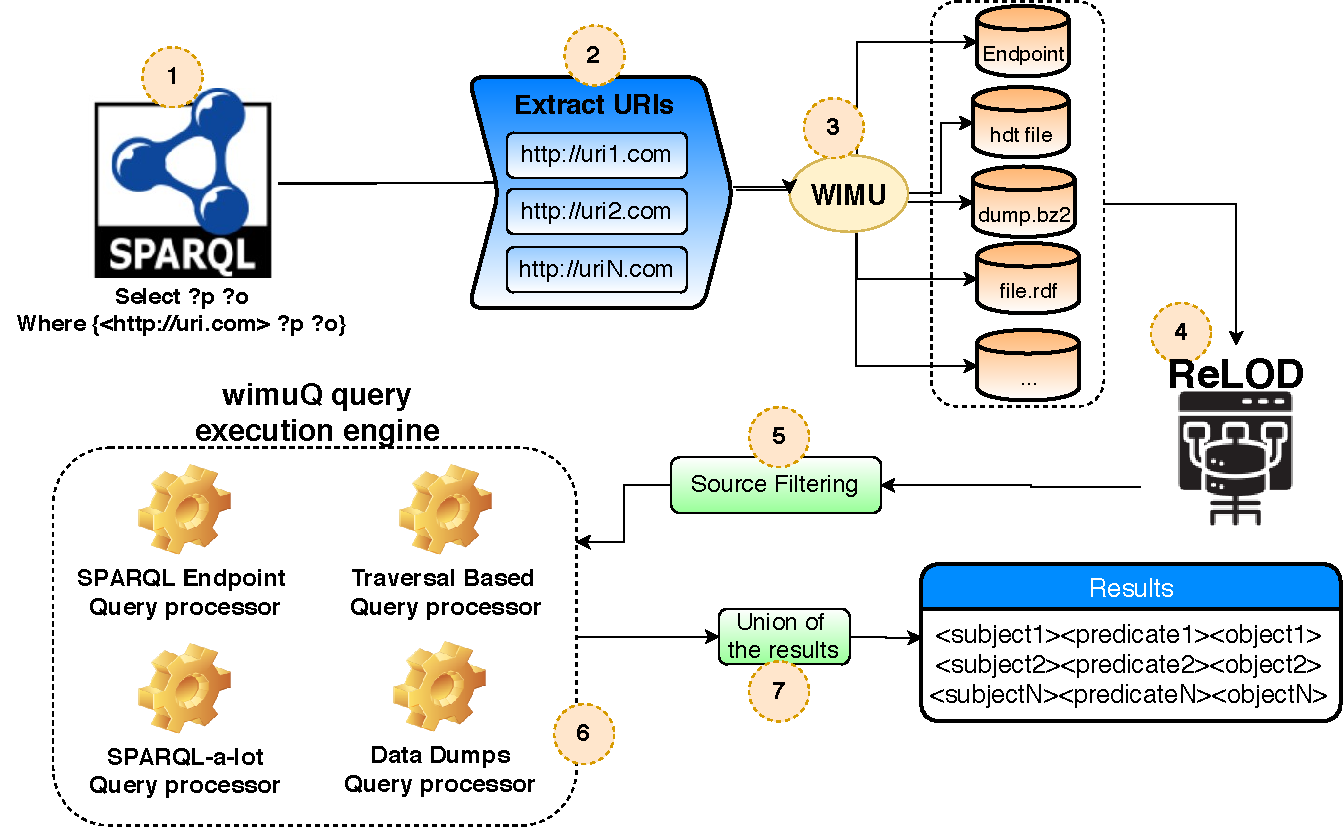
\includegraphics[width=0.8\linewidth]{img/wimuQ2.pdf}
	%\includegraphics[width=\linewidth]{img/wimuqArq.pdf}
	\caption{Query processing workflow.}
	\label{fig:approachWimuQ}
\end{figure*}

Now we go into the details of these steps, explaining the different components. 

\subsubsection{The source selection}
One of the important optimization steps in federated SPARQL query processing is the \emph{source selection} \cite{costfed2017,hibiscus2014}. The goal of the source selection is to identify the potentially relevant datasets (also called sources) to the given query. We make use of the WIMU service \cite{valdestilhas2018my} to select the potentially relevant sources. The WIMU service\footnote{WIMU URIs lookup service is available from: \url{http://wimu.aksw.org/}} provides URIs lookup facility and identify those datasets which contain the given URI. Currently, this service processed more than 58 billion unique triples and indexed 4.2 billion URIs from more than \SI{660}{\kilo\nothing} RDF datasets obtained from the most used Linked Data hubs including LODStats~\cite{auer2012lodstats} and LOD Laundromat~\cite{beek2014lod}. The identified WIMU datasets can be of four types: (1) SPARQL endpoint, (2) HDT file, (3) dataset with dereferenceable URIs, (4) data dump with non-dereferenceable URIs. 
The service is both available from a web interface as well as can be queried from a client application using the standard HTTP protocol.

\subsubsection{The query execution}
We make use of the four -- SPARQL endpoint, Link Traversal-based, SPARQL-a-alot, Data dumps -- query processor to execute federated queries over the aforementioned four types of WIMU datasets. The relevant data sources for each of these query processors are returned by the WimuQ source selection discussed in previous section. 

We used FedX \cite{fedx2011} query processor for SPARQL endpoints query federation and SQUIN for traversal-based query federation. The reason for choosing FedX for SPARQL endpoints federation and SQUIN for traversal-based federation is due the fact that they do not require any pre-computation of dataset statistics and hence are able to retrieve up-to-date results. Thus both are able to run federated queries with zero initial knowledge. In addition, both produce reasonably query runtime performances comparing to state-of-the-art approaches \cite{saleem2015fine,saleem2018costfed,hartig2013squin}.

The list of required endpoints URLs for FedX are returned from the previously discussed source selection Algorithm (ref. $\mathbf{E}$ of Algorithm \ref{alg:iss1}). The potentially relevant dereferenceable URIs data sources (ref. $\mathbf{T}$ of Algorithm \ref{alg:iss1}) are already identified by the WimuQ sources selection algorithm. Thus, we reduced the search space by only considering the dereferenceable URIs data sources. 
 
As mentioned before, FedX can only works with public SPARQL endpoints. SQUIN needs dereferenceable URIs. Both of these engines are unable to execute SPARQL queries over non-dereferenceable URIs datadumps: SPARQL endpoint federation approaches cannot execute queries over such datadumps as they are not exposed as SPARQL endpoints, link traversal-based approaches fail to retrieve results as the URIs are non-dereferenceable. We need to download the dumps first, load it locally, and run some query processing API (e.g., JENA or Sesame) on the loaded datasets. However, we can not simply download the complete dumps and process it locally due to their large amount of data. To solve this problem, we make use of the Wimu index to only select those data dumps which are potentially capable to execute the given query. These datadumps are further sliced by using the RDFSlice technique, to only select the required chunks of the datadumps which will provide results to the given SPARQL query. The identified chunks are finally loaded in a local Apache Jena model. The model is then use to execute federated queries. 

The results generated by each of WimuQ's processors are finally integrated and sent back to the user. 

\subsection{\textsc{ReLOD}---The incremental LOD Dataset relation index} \label{sec:relod}

Our observations guide us to a method to create an index of LOD datasets, in which involves a compilation of many other works, starting collecting data from more than \num{650000} LOD datasets from LODStats, LODLaundromat and more than 500 endpoints\footnote{The list of endpoints is available here: \url{https://github.com/firmao/wimuT/blob/master/Endpoints_numtriples_lodcloud.csv}}. 

%Among the steps we should hightlight the creation of a \textbf{Dataset catolog}, section\ref{sec:lodCatalog}, providing an efficient way to obtain all properties and classes from each dataset and an \textbf{approach to identify the namespace} of each dataset, described at section\ref{sec:namespace}, avoiding the necessity to open each dataset in order to know what more the domain of the dataset.

\subsection{The index creation}
\label{sec:indexCreation}

Given a set of Datasets $\mathbf{D}\{d_1,...,d_n\}$, assuming $d_n$ represents a RDF dataset\footnote{RDF datasets: \url{https://www.w3.org/TR/rdf11-datasets/}}, in which each $d$ contains a set of properties and classes represented by $\mathcal{P}$. The next step consists in creating a set $\mathbf{E}$ containing the identified duplicated datasets. Thus, we can exclude from $\mathbf{D}$ all datasets contained in $\mathbf{E}$.

The goal of algorithm \ref{alg:indexCreation}\footnote{Implementation in Java \url{https://tinyurl.com/y597qrah}} is to create an index to store the relations among datasets by comparing the occurrences of classes and properties of each dataset, by String similarity and Instance Matching. The \textbf{Input} is a set of Datasets and the \textbf{Output} is the index of dataset relations.

\cref{fig:create} shows a workflow about how the index is created and the algorithm \ref{alg:indexCreation} describe with more details the process of creation of the dataset relation index.

\begin{figure*}[htb] 
	\centering
	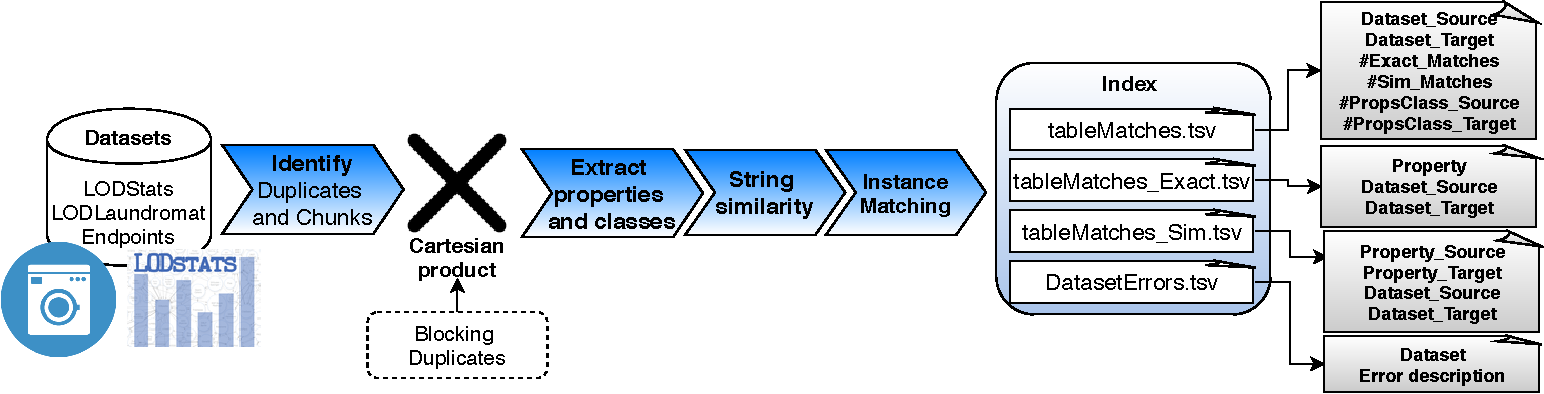
\includegraphics[width=\linewidth]{img/createIndex.pdf}
	\caption{Creating the index.}
	\label{fig:create}
\end{figure*}

\begin{figure*}[htb] 
	\centering
	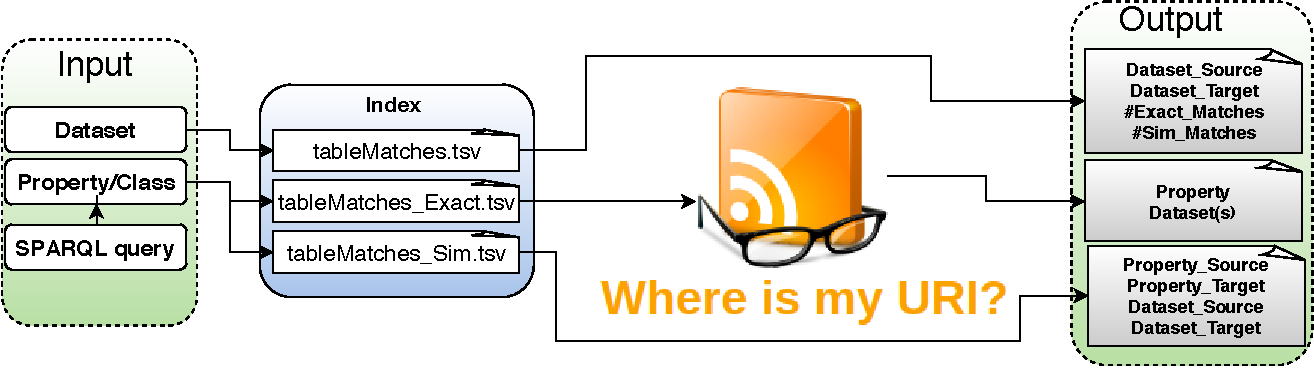
\includegraphics[width=\linewidth]{img/queryIndex.pdf}
	\caption{Querying the index.}
	\label{fig:queryIndex}
\end{figure*}

\begin{algorithm*} [htb] 
	\caption{Creation of the LOD dataset relation index}
	\label{alg:indexCreation}
    \begin{multicols}{2}
    	\textbf{Input}: $\mathbf{D}, \mathbf{E}$ \Comment{Datasets and datasets duplicated} \\
    	\textbf{Output}: $\mathbf{C}, \mathbf{X}, \mathbf{Y}, \mathbf{Z}$  \Comment{Four tsv files containing the matches(datasets, classes and properties).}
    	\begin{algorithmic}[1]
    	    \State{$\mathbf{M}_e \{\}$} \Comment{HashMap containing datasetTarget and another hash containing properties and classes exact matched}
    	    \State{$\mathbf{M}_s \{\}$} \Comment{HashMap containing datasetTarget and another hash containing properties and classes matched using String similarity}
    	    \State{$\mathbf{M}_a \{\}$} \Comment{HashMap containing datasets already compared}
    	    \State{$\mathbf{D}-\mathbf{E}$} \Comment{Remove duplicates contained in $\mathbf{E}$}
    	    \State{$\mathbf{T}=\mathbf{D}$}
    	    \ForAll{$\mathbf{d} \in \mathbf{D}$} \Comment{In parallel}
    	        \ForAll{$\mathbf{t} \in \mathbf{T}$}
        	        \If{($\mathbf{d}$ <> $\mathbf{t}$) $\land$ \textbf{alreadyCompared}($\mathbf{d},\mathbf{t}$)} 
        	            \State{continue} \Comment{Skip the current $\mathbf{d}$ and $\mathbf{t}$}
        	        \EndIf
        	        \State{$\mathbf{M}_e$.add(\textbf{getExactMatches}($\mathbf{d},\mathbf{t}$))} \Comment{Add a set containing the properties/classes that are exact the same in both datasets}
					\State{$\mathbf{M}_s$.add(\textbf{getSimMatches}($\mathbf{d},\mathbf{t}$, 0.8, $\mathbf{M}_e$))} \Comment{Add a set containing the properties that are similar in both datasets, excluding the matches from $\mathbf{M}_e$}
					\State{$\mathbf{M}_a$.add(d, t)} \Comment{Add the dataset pair already processed}
    	        \EndFor
    	    \EndFor
    	    \State{\textbf{printMaps}($\mathbf{M}_e, \mathbf{M}_s$)} \Comment{Print the content of $\mathbf{M}_e$ and $\mathbf{M}_s$ inside the files $\mathbf{C}, \mathbf{X}, \mathbf{Y}, \mathbf{Z}$}
    	\end{algorithmic}
    \end{multicols}	
\end{algorithm*}  

The function \textbf{getExactMatches}($\mathbf{d},\mathbf{t}$)) compares all properties and classes from each dataset $\mathbf{d}$ and $\mathbf{t}$ and return a set of properties and classes that are exact the same, keeping the provenance of the dataset.

The function \textbf{getSimMatches}($\mathbf{d},\mathbf{t}$, 0.8, $\mathbf{M}_e$) compares all properties and classes from each dataset $\mathbf{d}$ and $\mathbf{t}$ using Jaccard and MFKC\cite{valdestilhas2017high} String Similarity function with a threshold of 0.8, excluding the exact matches identified previously by the function \textbf{getExactMatches} returning a set of properties and classes that has the similary greater than the threshold 0.8, keeping the provenance of the dataset, the \cref{fig:simMatch} shows our string similarity process.
\begin{figure*}[htb] 
	\centering
	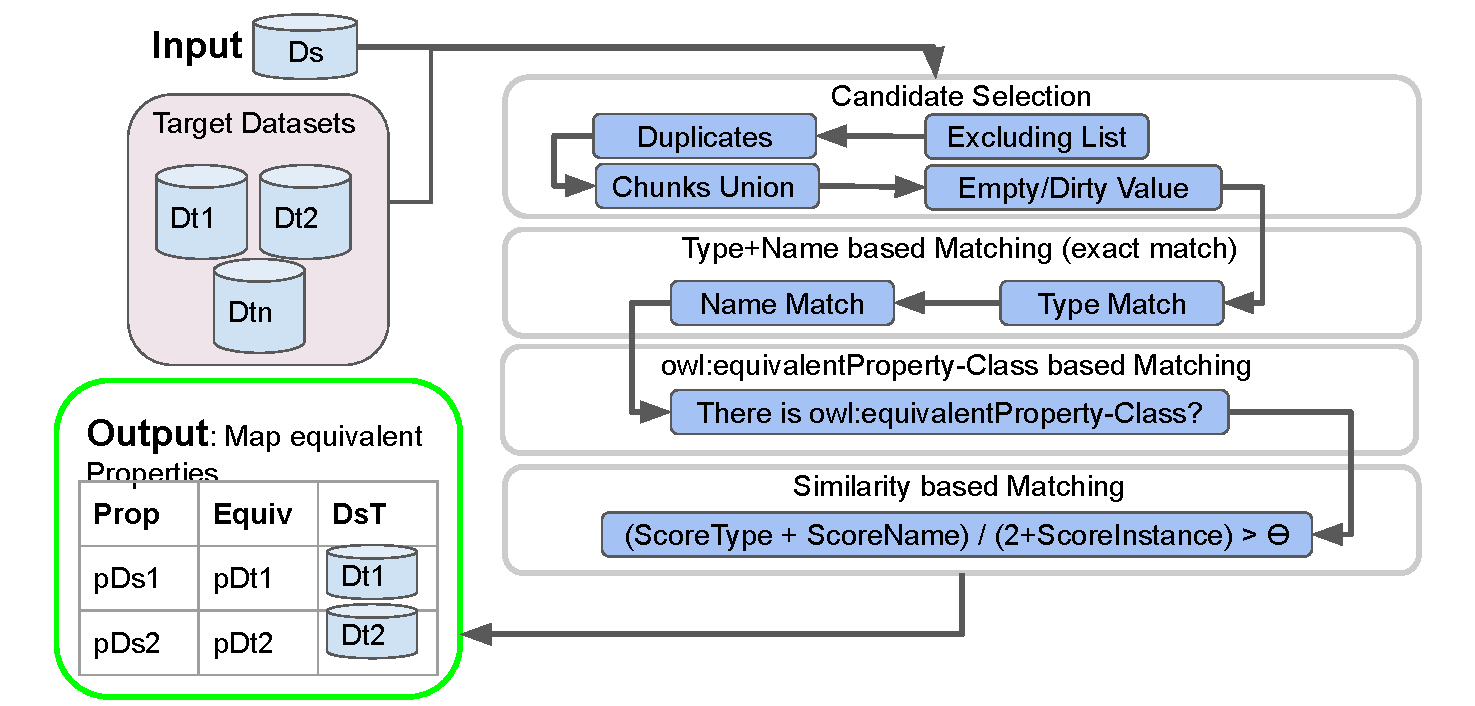
\includegraphics[width=0.8\linewidth]{img/stringSim.pdf}
	\caption{String similarity process.}
	\label{fig:simMatch}
\end{figure*}

The function \textbf{printMaps}($\mathbf{M}_e, \mathbf{M}_s$) print the content from the matching functions into the files according the structure described in section \ref{sec:FileStructure}.

\subsection{Identifying duplicated and chunk datasets}
\label{sec:duplicates}
With the current hardware available (HD 1Tb, Memory 16GB, processor intel core i7).
To compare all LOD datasets, in this case more than 600 thousand datasets, implies in more than 360 billion of comparisons($n \cdot n$), assuming that each comparison takes on average 1 millisecond, the whole operation will take more than 10 years.

Thus, we decided to have a blocking method to avoid unnecessary comparisons. To this aim, we create a way to detect duplicated and chunk-dump-files datasets, described on \cref{alg:iss1}. 
Our blocking method avoid datasets with less than 1 triple, duplicates, less than 5 properties, less than 5 classes.

The function \textbf{eliminateDuplicates()}, identify and eliminate duplicated HDT files by comparing the property occurrences of each dataset and the header metadata.

We formalize the problem of Clustering datasets identifying duplicates and chunks as follows:

We consider a set of $\mathbf{K}$ data sources $\mathbf{S_1}, . . . , \mathbf{S_k}$ containing property occurrences $\mathbf{O_1}, . . . , \mathbf{O_m}$. Each of property $\mathbf{P}$ is referenced by an \texttt{URI}, e.g., dbo:City\footnote{dbo:City states for the URI \url{http://dbpedia.org/ontology/City}}. Each $\mathbf{S}$ contains a header $\mathbf{H}$, with meta-data about the data in $\mathbf{S}$, such that $\mathbf{H} \subset \mathbf{S}$.

The goal is to create clusters of datasets $\mathbf{C}$ in two groups of elements from $\mathbf{K}$, in which are duplicates $\mathbf{D}$ and chunks $\mathbf{E}$, such that $\mathbf{D} \subset \mathbf{K} : \mathbf{E} \subset \mathbf{K} : \mathbf{K} \subset \mathbf{C}$.

We assume that all datasets are not empty and are RDF compatible with the HDT format.

Firstly we create a dense matrix of property occurrence and dataset. Then it was observed a standard in the dense matrix, that for some datasets the occurrence of the properties was exactly the same, as  \cref{fig:propOccurence} try to show a sample with 11 datasets, with 7 chunks identified\footnote{Those 11 datasets and the source are available here: \url{https://tinyurl.com/11chunkLaundromat}}. Then, we identify that we can put together those datasets to observe more characteristics.
In this second phase, we have a sub-collection of our initial collection of datasets and looking into the header metadata of those files we observe that for some files the meta-data is different. Then we have another sub-collection of files with different headers, and manually reading file by file we realize that they are chunks, in other words, part of a bigger dataset. 

\begin{figure*}[htb] 
    \centering
 	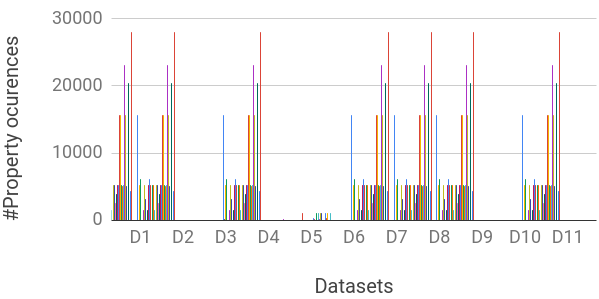
\includegraphics[width=0.8\linewidth]{img/propertyOccurence.png}
 	\caption{The standard observed in the dense matrix, showing that for some datasets the occurrence of the properties was exactly the same, in this case a sample with 11 datasets with 7 dataset chunks identified.}
 	\label{fig:propOccurence}
\end{figure*}

Thus we have two phases for clustering dataset (1) Put together datasets that present the same occurrence of properties. (2) Read the header metadata and separate files with a different header. The files with different header are chunks and the rest are duplicates\footnote{More details, please see the implementation and the documentation on \url{https://github.com/firmao/wimuT} and the specific implementation java class for this task: \url{https://github.com/firmao/wimuT/blob/master/src/org/wimu/datasetselection/parallelv1/ClusterKmeans.java}}.

% \begin{figure}[htb] 
% 	\centering
% 	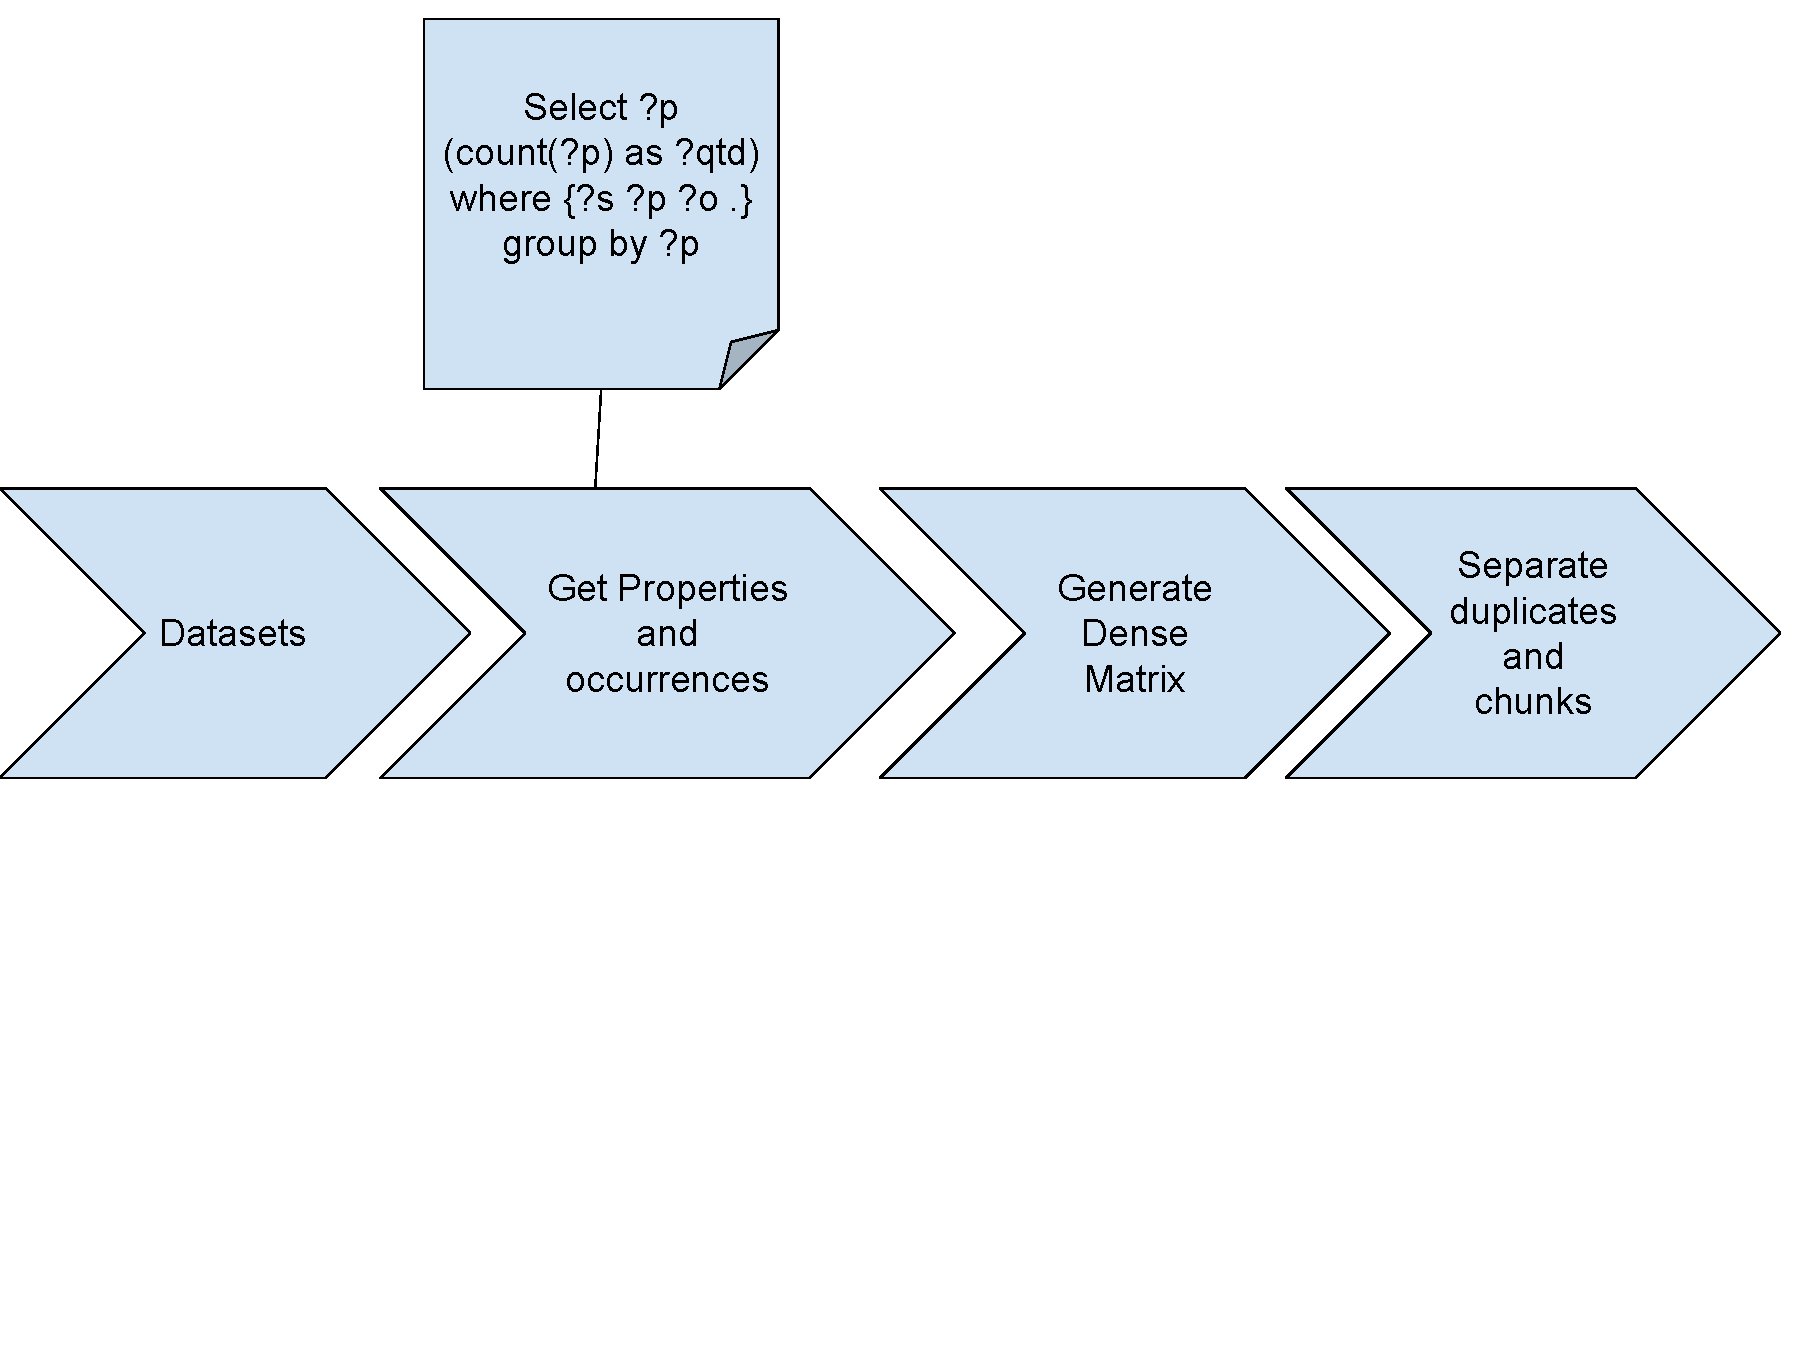
\includegraphics[width=\linewidth]{img/duplicates.pdf}
% 	\caption{Identifying duplicates and chunks.}
% 	\label{fig:duplicates}
% \end{figure}

\begin{algorithm*} [htb] 
	\caption{Identifying duplicates and chunk}
	\label{alg:iss1}
    \begin{multicols}{2}
    	\textbf{Input}: $\mathbf{D}$ \Comment{Datasets} \\
    	\textbf{Output}: $\mathbf{C}, \mathbf{X}$  \Comment{two files chunks.txt and duplicates.txt.}
    	\begin{algorithmic}[1]
    	    \State{sep = $\mathbf{t}$} \Comment{Separator for the file, in this case, a tab, but could be another such as “,”, etc..}
    	    \State{setHeader = $\{\}$}
    	    \State{cSparql = “Select ?p (count(?p) as ?qtd) where {?s ?p ?o .} group by ?p”}
    	    \ForAll{$\mathbf{d} \in \mathbf{D}$}
    	        \State{H = getPropertyOccurrence(ds)}
    	        \ForAll{$\mathbf{key,value} \in \mathbf{H}$} \Comment{\textbf{key} represent the property and \textbf{value} represents the number of occurrences.}
    	            \State{setHeader.add(key)}
    	            \State{line = line + sep + value}
    	        \EndFor
    	        \State{printLineDenseMatrix(d + line)}
    	        \If{setLines.contains(line)} \Comment{Here we identify and put chunks and duplicates together}
    	            \State{$\mathbf{D’}$.add(d)}
    	        \Else
    	            \State{setLines.add(line)}
    	        \EndIf
    	    \EndFor
    	    \State{printHeaderDenseMatrix(setHeader)}
    	    \State{$\mathbf{C}$.add(diff($\mathbf{D’}$))} \Comment{Here we separate chunks and duplicates}
    	    \State{$\mathbf{X}$.add(diffD($\mathbf{D’}$))}
     		\State{return $\mathbf{C}, \mathbf{X}$} \Comment{two files chunks.txt and duplicates.txt.}
    	\end{algorithmic}
	\end{multicols}
\end{algorithm*}    	

The function \textbf{getPropertyOccurrence}(ds) returns a hash map containing the property and the number of occurrences of each property from a given dataset with the SPARQL query at \cref{lst:propOccur1} 

\begin{lstlisting}[language=SPARQL, label={lst:propOccur1}, caption=Property occurrence query.]
Select ?p (count(?p) as ?qtd) where {?s ?p ?o .} group by ?p
\end{lstlisting}
The function \textbf{printLineDenseMatrix}(line) print a line in a file and the function \textbf{printHeaderDenseMatrix}(setHeader) print the first line of the dense matrix file containing the header of the matrix, in which refers to the identification of the properties.
The function \textbf{diff}($\mathbf{D’}$ ) separates the chunks from duplicates, for this task we look into the header of the files, in this case, only HDT files, where duplicates present exactly the same header metadata information and chunks are different respect to the header.

\textbf{Theorem 1}: Let $\mathbf{P}$ be a collection of property occurrences of datasets $\mathbf{D}$, such that each $\mathbf{D}$ has one $\mathbf{P}$, in which $\mathbf{D’}$ represents the cluster candidates, in which are the datasets identified as chunks and duplicates together, and the function \textbf{diff()} return the dump-files that are not duplicated. Thus, the output of Algorithm 1 when applied to $\mathbf{D}$, the following hold:

$|\textbf{diff}(\mathbf{D’})| = 0$

All elements from $\mathbf{D’}$ are duplicated datasets.


To identify the chunks:

$|\textbf{diff}(\mathbf{D’})| > 0$


The result from $\textbf{diff}(\mathbf{D’})$ are the dump-files identified as chunks.

% \subsection{The LOD catalog - Class property index}
% \label{sec:lodCatalog}
% \todo[inline]{Claus, when you are ready let's put your work here and some experiments/evaluation later. I also need to adapt my code to yours.}

% \subsection{Relating the name spaces with dataset names}
% \label{sec:namespace}
% The datasets from LODLaundromat\cite{} are identified with a MD5 code\footnote{ref MD5}, e.g \texttt{009e80050fa7f4279596956477157ec2.hdt}\footnote{\url{http://139.18.13.76:8082/dirHDTLaundromat/decompressed/00/009e80050fa7f4279596956477157ec2/009e80050fa7f4279596956477157ec2.hdt}} represent a dataset from the domain \texttt{knoesis.wright.edu} in which is a dataset about \textit{The Ohio Center of Excellence in Knowledge-enabled Computing (Kno.e.sis)}.

% We developed a method to convert the MD5 code from the HDT to URLs with more informative name spaces, instead of the MDA code we have the name space of the dataset giving us more information about the dataset avoiding the need to open the HDT file to obtain this information.

% The Algorithm \cref{alg:Edgard} describes how we create this complementary index.

% \todo[inline]{Edgard, please describe the algorithm when is better for you. And some evaluation.}

% \begin{table}[]
% \begin{tabular}{@{}lcccc@{}}
% \toprule
% \textbf{Process}           & \multicolumn{1}{l}{\textbf{Runtime}} \\ \midrule
%  Complete Namespace extraction & ?             \\              
%  Dominant Namespace extraction & ?             \\              Index creation    & ?               \\
%  \bottomrule
% \end{tabular}
% \end{table}

\subsection{The file structure}
\label{sec:FileStructure}

Now we describe the file structure that we created to use our index, which consists of 3 TSV\footnote{Tab Separated Value(TSV)} files.
\begin{itemize}
    \item $\textbf{tableMatches\_Exact.tsv}$: Contains the exact match of the properties, with the following fields: 
    \begin{itemize}
        \item \textbf{Property}: containing the property URI itself.
        \item \textbf{Source}: Contains the dataset source where the property was found.
        \item \textbf{Target}: Contains de dataset matched containing the property.
    \end{itemize}
    \item $\textbf{tableMatches\_Sim.tsv}$: Represents the similarity of properties from datasets Source and Target, with the following fields:
    \begin{itemize}
        \item \textbf{PropertyS}: The property from the dataset Source.
        \item \textbf{PropertyT}: The property from the dataset Target.
        \item \textbf{Source}: The dataset Source.
        \item \textbf{Target}: The dataset Target.
    \end{itemize}
    \item \textbf{tableMatches.tsv}: Represents the datasets Matched and his respectives number of properties exact matched and number of properties matched with String similarity, with the following fields:
    \begin{itemize}
        \item \textbf{Source}: The dataset source.
        \item \textbf{Target}: The dataset Target.
        \item $\textbf{\#ExactMatch}$: Number of properties with exact match.
        \item $\textbf{\#sim>0.9}$: Number of properties with similarity threshold greater than 0.9.
    \end{itemize}
\end{itemize}

\subsection{Querying the index}
%\todo[inline]{Describe how to query the index, how the web prototype do the task: \url{https://github.com/firmao/LODDatasetRelationsWeb}} 

The index provides the following information based on three types of input:
\begin{description}
    \item \textbf{Dataset}: The index will provide a list of datasets, number of exact matched\footnote{Exact Match where the URI is exact the same following the principle of uniqueness of the URI} properties and number of similar\footnote{Similarity match occurs when the similarity of the URI is greater than 0.9 if less we perform Instance matching.} properties.
    \item \textbf{Set of properties (URIs) separeted by comma}: 
    \begin{itemize}
        \item Json file containing the property and the list of datasets where this property were found by exact match.
        \item A table containing the matches by similarity with the following fields:
        \begin{description}
            \item \textbf{Property Source}: Representing the property found on the dataset source.
            \item \textbf{Property Target}: Representing the property found on the dataset target.
            \item \textbf{Dataset Source}: The name of the dataset source.
            \item \textbf{Dataset Target}: The name of the dataset target.
        \end{description}
    \end{itemize}
    \item \textbf{SPARQL query}: This type of input extracts the set of properties from the SPARQL query and performs the same operation as \textbf{Set of properties (URIs) separeted by comma}.
\end{description}

The index is also incremental, allowing to add more datasets to be processed once a month\footnote{Once a month due to the the time to generate that with our hardware takes at least 88 hours}.
The prototype is available online for proof of concept online\footnote{\url{http://w3id.org/relod/}} and the \cref{fig:queryIndex} shows a workflow about how the index is used.



% \todo[inline]{try with elasticsearch and see if is better or not.}
% \begin{verbatim}
% elasticsearch_loader <options> csv --delimiter '\t' filename.tsv

% https://www.reddit.com/r/elasticsearch/comments/at7huu/how_can_i_import_tsv_to_elasticsearch/
% \end{verbatim}

%The \cref{fig:datasetMatch},\cref{fig:exactMatch}, \cref{fig:similarMatch} show 3 examples of 3 different types of results to 3 different queries to the index.

% \begin{figure}[htb] 
% 	\centering
% 	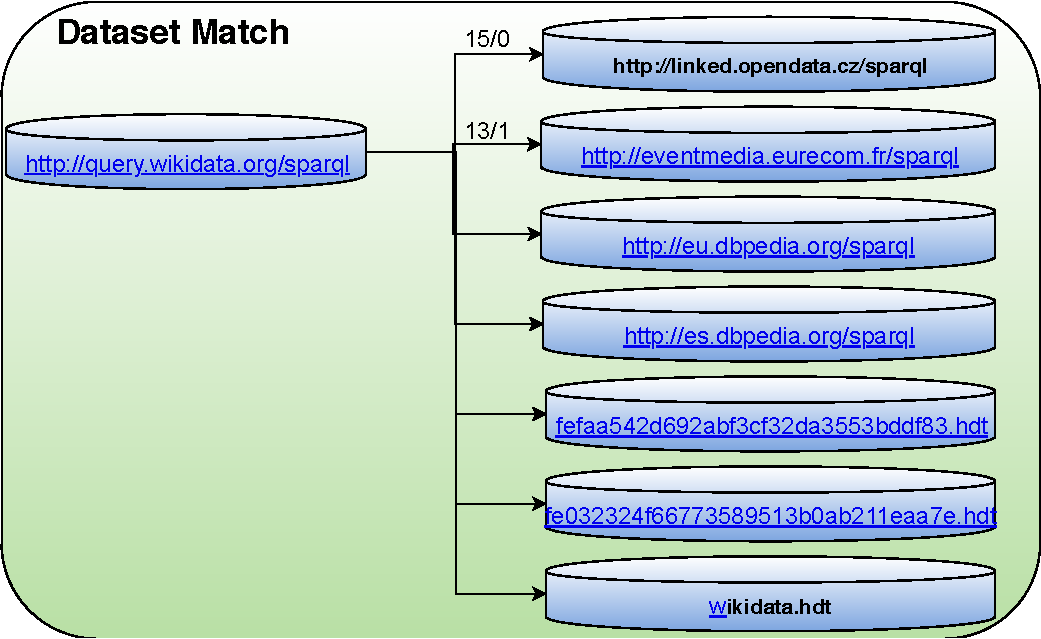
\includegraphics[width=\linewidth]{img/datasetMatch.pdf}
% 	\caption{Example of dataset match.}
% 	\label{fig:datasetMatch}
% \end{figure}

% \begin{figure}[htb] 
% 	\centering
% 	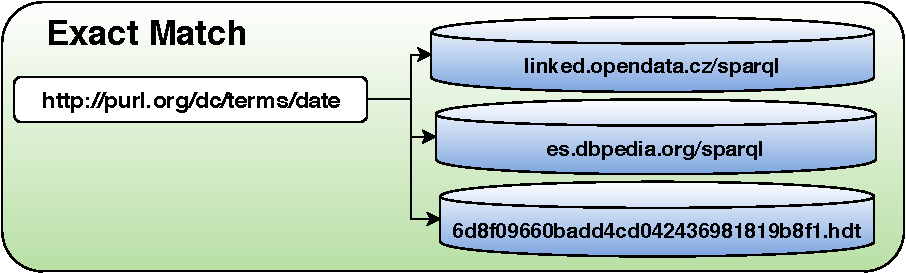
\includegraphics[width=\linewidth]{img/exactMatch.pdf}
% 	\caption{Example of exact match.}
% 	\label{fig:exactMatch}
% \end{figure}

% \begin{figure}[htb] 
% 	\centering
% 	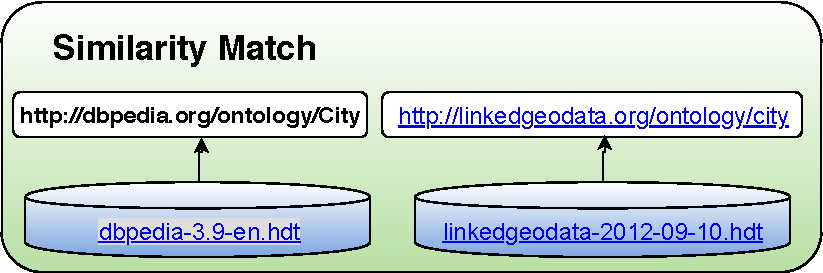
\includegraphics[width=\linewidth]{img/similarMatch.pdf}
% 	\caption{Example of similar match.}
% 	\label{fig:similarMatch}
% \end{figure}

\begin{table*}[htb]
\centering
\caption{Sample datasets from \cite{georgala2018dynamic} to evaluate our string similarity approach.}
\label{tab:TableFmeasure}
\resizebox{1.0\textwidth}{!}
{
\begin{tabular}{*{6}{c}} \hline
    \textbf{Data set}           & \textbf{Source (S)} & \textbf{Target (T)} & \textbf{$|S| \times |T|$} & \textbf{Source Property} & \textbf{Target Property}                           \\ \hline
    
    \textbf{(P3)}Abt-Buy    & Abt & Buy  & $1.20 \times 10^6$ & product name, description                       & product name, description                         \\
                                &&&& manufacturer, price               & manufacturer, price                       \\ \hline
    \textbf{(P4)}Amazon-GP  & Amazon & Google & $4.40 \times 10^6$ & product name, description                 & product name, description                         \\ 
                                && Products && manufacturer, price               & manufacturer, price                       \\ \hline
    \textbf{(P5)}DBLP-ACM  & ACM & DBLP& $6.00 \times 10^6$ & title, authors                    & title, authors                            \\
                                &&&& venue, year                       & venue, year                               \\ \hline
    \textbf{(P6)}DBLP-Scholar& DBLP & Google  & $ 0.17 \times 10^9$ & title, authors                    & title, authors                            \\
                                && Scholar && venue, year                       & venue, year                               \\ \hline
    \textbf{(P7)}MOVIES   & DBpedia & LinkedMDB & $0.17 \times 10^9$ & dbp:name                          & dc2:title     \\
                                &&&& dbo:director/dbp:name             & movie:director/movie:director\_name       \\
                                &&&& dbo:producer/dbp:name             & movie:producer/movie:producer\_name       \\
                                &&&& dbp:writer/dbp:name            & movie:writer/movie:writer\_name           \\
                                &&&& rdfs:label & rdfs:label           \\ 
                                \hline
\end{tabular}
}
\end{table*}

\section{Evaluation}
\label{sec:eval}

\subsection{Evaluation on Identifying LOD datasets}

To the best of our knowledge, LODStats\cite{auer2012lodstats} is the only project oriented to monitoring dump files; however, its last update dates back to 2016. 
Observing \Cref{tab:lodstats}, we are able to say that from LODStats, not all datasets are ready to use.
Especially, more than 58\% are off-line, 14\% are empty datasets, 8\% of the triples that have literals as objects are blank nodes and 35\% of the online datasets present some error using the Apache Jena parser\footnote{See \url{https://github.com/dice-group/wimu/blob/master/ErrorJenaParser.tsv}.}. 
A large part of those data was processed and cleaned by LOD Laundromat~\cite{beek2014lod}.


\setlength{\tabcolsep}{0.1em} % for the horizontal padding
\begin{table}[H]
	\centering
	\caption{Datasets.}
	\label{tab:lodstats}
    \begin{tabular}{|l|r|r|r|}
    \hline
    & \textbf{LOD Laundromat} & \textbf{LODStats} & \textbf{Total} \\ 
    \hline
    \textbf{URIs indexed} & \num{4185},\num{133445} & \num{31121342} & \num{4216254787} \\ \hline
    \textbf{Datasets checked} & \num{658206} & \num{9960} & \num{668166} \\ \hline
    \textbf{Triples processed} & \num{19891702202} & \num{38606408854} & \num{58498111056} \\
    \hline
    \end{tabular}
\end{table}

The algorithm took three days and seven hours to complete the task. 
Thus, we will create a scheduled job to update our database index once a month.
With respect to the information present in the \cref{fig:dumps}, we can observe that the majority of files from LODStats are in RDF/XML format.
Moreover, the endpoints are represented in greater numbers (78.6\%), the dominant file format is RDF with 84.1\% of the cases, and 56.2\% of errors occurred because Apache Jena was not able to perform SPARQL queries.
Among the HDT files from LOD Laundromat, 2.3\% of them could not be processed due to parsing errors.
Another relevant point is that 99.2\% of the URIs indexed with WIMU come from LOD Laundromat, due to 69.8\% of datasets from LODstats contain parser errors in which WIMU was not able to process the data.
%https://docs.google.com/spreadsheets/d/15kh8E4WllXG5Xdp1aL-JiHvnXAiVC6a8XqVUJ1gtMZ8/edit?usp=sharing

\begin{figure*}[htp] 
	\centering
	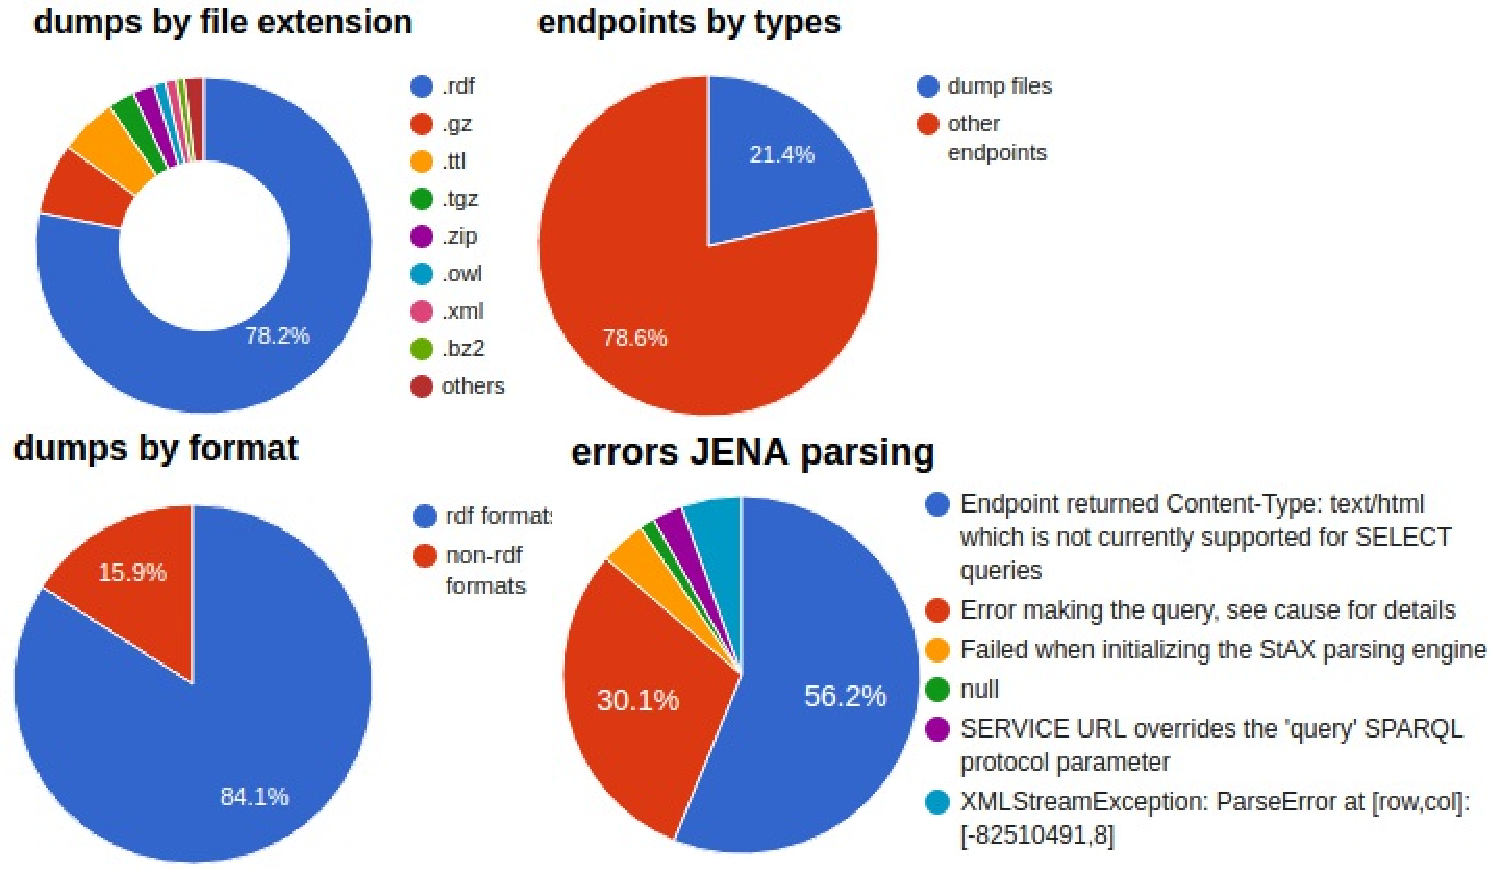
\includegraphics[width=0.9\textwidth]{img/dumps3.pdf}
	\caption{Dump files and Apache Jena parsing error.}
	\label{fig:dumps}
\end{figure*}

Finally, we validated our heuristic assessing if the URI really belongs to the dataset with more literals.
To this end, we took a sample of 100 URIs\footnote{\url{https://github.com/dice-group/wimu/blob/master/result100.csv}} that belong to at least two datasets, where we assess manually the data in order to check if the results are really correct. 
As a result, the dataset containing the correct information was found as first result in 90\% of the URIs and among the top three in 95\% of the URIs.

To see how and where people are using WIMU the \cref{fig:wimuUsage} shows the usage of WIMU by country, where we have \num{63526} number of queries, using \num{35984} URIs, in which \num{35918} are valid URIs. The data was collected from December 2018 until February 2020. 

\begin{figure}[htp] 
	\centering
	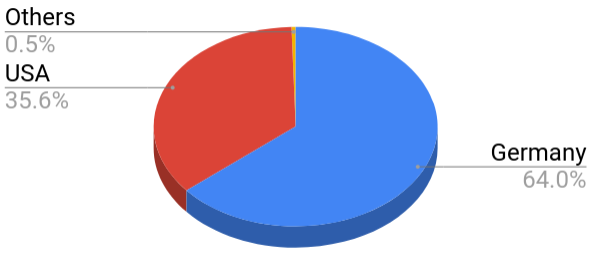
\includegraphics[width=\linewidth]{img/wimuUsage.png}
	\caption{The usage of WIMU.}
	\label{fig:wimuUsage}
\end{figure}

%\todo[inline]{ED: Change the name on Figure 7 from Brazil to Others}

\subsection{Evaluation on Querying and source selection LOD datasets}
In this section, we present the evaluation setup and the corresponding results that validate our hypothesis that we can improve the resultset retrieval if we automatically identify potentially relevant sources from heterogeneous RDF data even if the URIs are not dereferenceable anymore. The goal of this evaluation is to show that by combining different SPARQL query processing approaches, we are able to retrieve more complete results as compared to the results retrieved by the individual approaches. 
\subsection{Experimental setup}

\subsubsection{Benchmarks used:} Since WimuQ aims to execute SPARQL queries over real-world RDF datasets, we chose three -- FedBench \cite{fedbench2011}, LargeRDFBench \cite{largerdfbench2017}, Feasible \cite{feasible2015} -- real-world RDF datasets benchmarks in our evaluation: 
\begin{itemize}
  
\item \textbf{FedBench} is federated SPARQL querying benchmarks. It comprises of a total of 25 queries and 9 real-world interconnected datasets. FedBench queries are further divided into three main categories: (1) 7 queries from Life Sciences (LS) domain, (2) 7 queries from Cross Domain (CD), and (3) 11 queries named Linked Data (LD) for link traversal-based approaches. The detailed statistics of the benchmark's datasets and queries are given in FedBench\cite{fedbench2011}.

\item  \textbf{LargeRDFBench} is also a federated SPARQL querying benchmark. It comprises a total of 40 queries and 13 real-world interconnected datasets. FedBench queries are further divided into four main categories: (1) 14 \emph{Simple} queries, (2) 10 \emph{Complex} queries, (3)  8 \emph{Large Data} queries, and (4) 8 \emph{Complex+High Data Sources} queries. The detailed statistics of the benchmark's datasets and queries are given in \cite{largerdfbench2017}. 

\item  \textbf{FEASIBLE} is a benchmark generation framework which generates customized benchmarks for the queries logs. In our evaluation, we chose exactly the same benchmarks used in \cite{feasible2015}: (1) 175 queries benchmark generated from DBpedia queries log and (2) 175 queries benchmark generated from Semantic Web Dog Food (SWDF) queries log. Further advanced statistics of the used datasets and queries can be found in \cite{feasible2015}. 
\end{itemize}
To the best of our knowledge, these are the state-of-the-art from the real-data SPARQL benchmarks. All of the 415 queries used in our evaluation is publicly available\footnote{Queries available from \url{https://github.com/firmao/wimuT/blob/master/queriesLocation.txt}}. 

\subsubsection{Hardware:} All the experiments were done on a modest machine with 200 GB of Hard Disk, 8 GB of RAM and a 2.70GHz single core processor. Each of the queries was run 5 times and the average of the results are presented.  

\subsubsection{SPARQL endpoints:} As previously stated, the query federation over multiple SPARQL endpoints approaches requires the set of endpoint URLs to be provided as input to the federation engine. We chose a total of 539 active SPARQL endpoints available from LOD cloud\footnote{List of SPARQL endpoints: \url{https://lod-cloud.net/lod-data.json}}. We filtered the endpoints URLs\footnote{\label{endpoints}Endpoints URLs with size: \url{https://goo.gl/H2t5ko}} and the total number of triples hosted by each of these endpoints. 

\subsubsection{Metrics:} Since WimuQ aims to retrieve more complete results within the reasonable amount of time, we choose two metrics: (1) coverage in terms of the number of results retrieved from the query executions and (2) the time taken to execute the benchmark queries. 

\subsubsection{Approaches:} As mentioned in Section \ref{sec:related}, different federation engines available to federate SPARQL queries over endpoints and traversal-based federation. We chose FedX \cite{fedx2011} for SPARQL endpoint federation and SQUIN \cite{hartig2013squin} for traversal-based query federation. The reason for choosing these two engines is due the fact they do not require any pre-computation of dataset statistics and hence able to retrieve up-to-date results and able to run federated queries with zero initial knowledge. In addition, both these engines perform reasonably well in terms of query runtime performances w.r.t state-of-the-art approaches \cite{saleem2015fine,saleem2018costfed,hartig2013squin}. For the sake of completeness, we also compared WimuQ with SPARQL-a-lot and WimuDumps.  

%In total, we processed more than 5 Terabytes of information from datasets retrieved using WIMU. None of ours experiment SPARQL query setups occupied more than 200 GB in disk. The source-code to reproduce the experiments is available online\footnote{\url{https://github.com/firmao/wimuT}}.
%In case, the machine do not need to have more than 200 GB, because we start discarding the datasets when reach the limit of 200 GB according to the use
\subsubsection{Results}
\textbf{Coverage of the results}: The main purpose of WimuQ is to devise a federation engine which is able to retrieve more complete results for the given SPARQL queries. %One of the most important results is the coverage of the results achieved by using each selected methods to compose the WimuQ. 
\Cref{fig:numberRes1} shows a comparison of the selected approaches in terms of the average of the number of results retrieved for the different queries categories of the selected benchmarks. The complete results for individual queries can be found on our aforementioned project website. By using different query processing engines, our approach is able to retrieve more results as compared to the results retrieved by only using SPARQL endpoints federation engine (i.e, FedX) link traversal engine (i.e., SQUIN), data dumps, or  HDT files. In our evaluation, the average resultset size of WimuQ is \num{8481} across the three benchmarks. Out of these, WimuQ collects about 91\% of the results from wimuDumps (avg. resultset size 7651), 7\% from SPARQL endpoints (avg. resultset size 556), and 1\% from SPARQL-a-lot (avg. resultset size 74). 

\begin{figure*}[htb]
    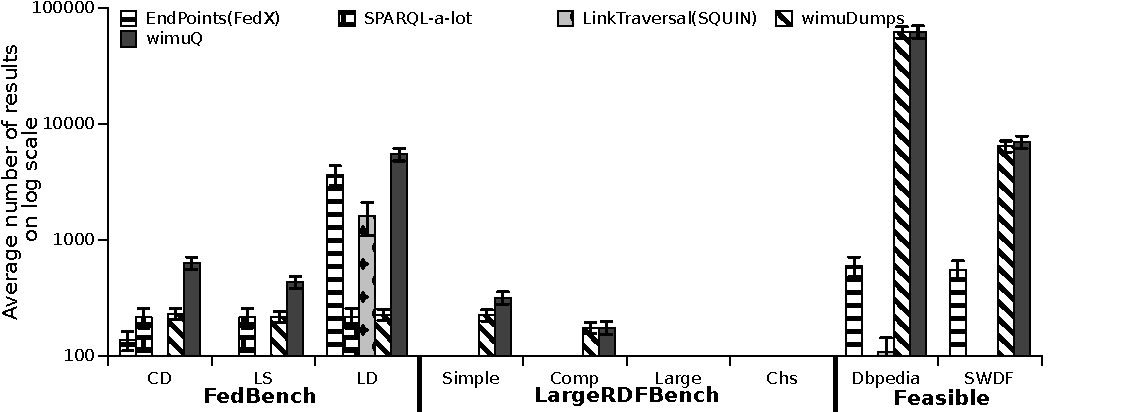
\includegraphics[width=\textwidth]{img/numberRes1.pdf}
	\caption{Average number of results retrieved by the selected approaches across different queries categories of the selected benchmarks.}
	\label{fig:numberRes1}
\end{figure*}

For FedBench, the WimuQ avg. resultset size is \num{2253}. Out of these results, about 55\% are collected from SPARQL endpoints by using FedX query processing engines (avg. resultset size \num{1262}). The LinkTraversal (SQUIN) contributed about 25\% of the total results (avg. resultset size 549), wimuDumps contributed about 10\% of the total results (avg. resultset size 226), and SPARQL-a-lot also contributed about 10\% of the results (avg. resultset size 215). 

For LargeRDFBench, the WimuQ avg. resultset size 123. Out of these results, about 81\% are collected from wimuDumps (avg. resultset size 100). The SPARQL endpoints contributed about 14\% of the results (avg. resultset size 17). The LinkTraversal(SQUIN) contributed 6\% of the total results (avg. resultset size 6), and SPARQL-a-lot did not provide results (avg. resultset size 0). 

For FEASIBLE, the WimuQ avg. resultset size \num{34537}. Out of these results, about 98\% are collected from wimuDumps (avg. resultset size \num{33893}). The SPARQL endpoints contributed about 1.6\% (avg. resultset size 577). The LinkTraversal(SQUIN) approach contributed only about 0.15\% (avg. resultset size 54). Finally, SPARQL-a-lot query processing engine only retrieved about 0.03\% results (avg. resultset size 11). 

In summary, WimuQ is able to retrieve at least one resultset for 76\% of the overall 415 queries. The results clearly shows that by combining different query processing engines into a single SPARQL query execution framework lead towards more complete resultset retrieval. 
An important observation is that the selected approaches are mostly not able to retrieve results for the Large Data and Complex+High (Ch) queries categories of LargeRDFBench. The reason is getting zero results for the Large Data queries is that these queries retrieve results from the LinkedTCGA \cite{tcga2013} datasets which were not publicly available via SPARQL endpoints, were not indexed by WIMU, also were not reachable via link traversals. While Ch queries often require higher number of distributed datasets in order to compute the final resultset of the queries. Thus, the approaches were able to find all of the relevant datasets, required to compute the final resultset of the queries. The average number of datasets\footnote{Here we also point the number of datasets discovered} queries by WimuQ for the selected benchmarks queries categories in given in Figure \ref{fig:numberDatasets1}. We can clearly see the highest number of datasets are selected for Ch queries of LargeRDFBench. 

\begin{figure*}[htb]
\centering
    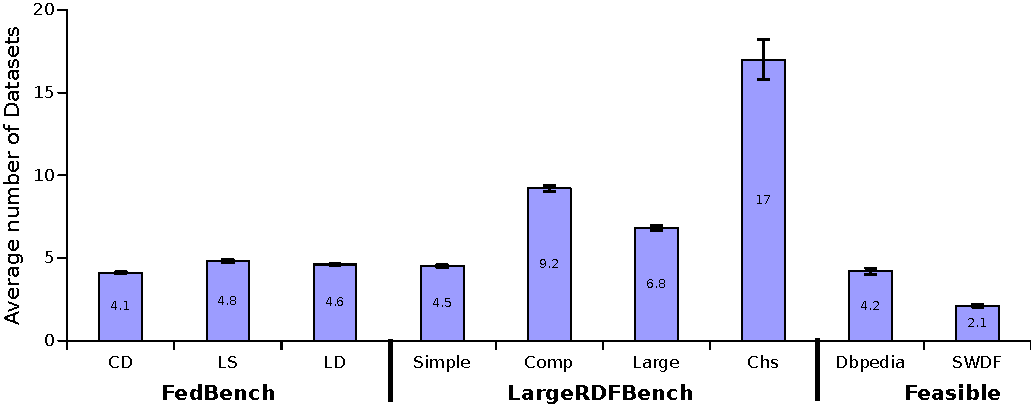
\includegraphics[width=0.9\textwidth]{img/numberDatasets1.pdf}
	\caption{Average number of datasets discovered and queried by WimuQ across different queries categories of the selected benchmarks.}
	\label{fig:numberDatasets1}
\end{figure*}

\textbf{Query runtime performances}: 
\Cref{fig:runtime1} shows a comparison of the selected query processing engines in terms of the average query run times for the different queries categories of the selected benchmarks. The average query runtime of WimuQ is 17 minutes across the three benchmarks. The average query execution to collect results from wimuDumps is about 2 minutes, which in turn is followed by query execution over SPARQL endpoints (avg. query runtime 13 minutes), SPARQL-a-lot (avg. query runtime 58 seconds) and LinkTraversal (SQUIN) (avg. query runtime 36 seconds). Interestingly, WimuQ collects about 91\% of the results from wimuDumps yet its average execution time is smaller than query execution over SPARQL endpoints which provide only 7\%  of the total results. One possible reason for this could be that in SPARQL endpoint federation, the query processing task split among multiple selected SPARQL endpoints and hence network and the number of intermediate results play an important role in the quer runtime performances. 

For FedBench, the WimuQ average query runtime 20 minutes. Out of this, the average avg. query runtime over SPARQL endpoints is 16 minutes, followed by wimuDumps (avg. query runtime 2 minutes), LinkTraversal (SQUIN) (avg. query runtime 49 seconds), and SPARQL-a-lot (avg. query runtime 46 seconds), respectively. For LargeRDFBench, the average query execution of WimuQ is 11 minutes. Out of this query execution over SPARQL endpoints took 8 minuts on average, followed by wimuDumps (avg. query runtime 2 minutes), SPARQL-a-lot (avg. query runtime 35 seconds), and LinkTraversal (SQUIN) (avg. query runtime 25 seconds), respectively. For FEASIBLE, the WimuQ takes on average of 24 minutes per query execution. Out of this, the query federation over SPARQL endpoints took about 18 minutes on average. Which is followed by wimuDumps (avg. query runtime 3 minutes), SPARQL-a-lot (avg. query runtime 1), and LinkTraversal (SQUIN) (avg. query runtime 36 seconds), respectively.

As an overall query runtime evaluation, we can clearly see there is a trade-off between the recall and query runtimes: the highest the recall the highest the query runtimes. Finding a balance between the recall and runtime would be an interesting research question to be considered in the future.  

\begin{figure*}[htb]
    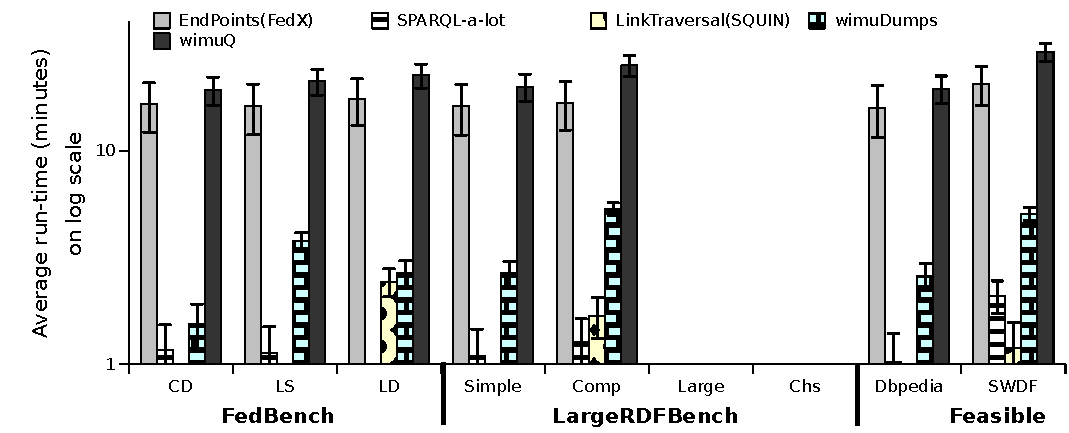
\includegraphics[width=\textwidth]{img/runtime1Min.pdf}
	\caption{Average query runtimes of the selected approaches across different queries categories of the selected benchmarks.}
	\label{fig:runtime1}
\end{figure*}

The results of our evaluation lead us to validate our hypothesis that we can improve the resultset retrieval if we identify potentially relevant sources from heterogeneous RDF data.

\subsection{Evaluation on Relating LOD datasets} \label{sec:relod_eval}
% The evaluation aims to answer the following questions: (1) How to identify and quantify similar datasets for a given Dataset?\footnote{To know how many datasets are similar to each other.} (2) How many datasets are most likely to execute a given SPARQL query? (3) How many datasets you should read the content to know the domain and namespace? (4) How the detection of duplicated and chunk datasets can help in the process of matching a large amount of datasets?
This evaluation aims to answer the following questions: (1) How to identify and quantify similar datasets for a given Dataset?\footnote{To know how many datasets are similar to each other.} (2) How many datasets are most likely to execute a given SPARQL query? (3) How the detection of duplicated and chunk datasets can help in the process of matching a large amount of datasets? (4) How ReLOD increase the number of datasets identified by wimuQ?


The information contained at \cref{tab:simJaccard} and \cref{tab:contained} are used to see how a sample of datasets are similar, we take 8 famous datasets from \textit{rdfhdt.org}\footnote{\url{http://www.rdfhdt.org/datasets/}} and 12 from \cite{10.1145/3308560.3317075}. To obtain the results from the \cref{tab:simJaccard}. which is to see how similar are the datasets, we use the formula \cref{eq:jaccard} and to obtain the results from \cref{tab:contained}, to see how much a dataset is contained inside each other we use the formula in \cref{eq:contained}, in this way, normalizing the similarity score between 0 and 1, where A and B represent datasets source and target. We have an alternative way to visualize this sample data as a graph\footnote{\url{https://w3id.org/relod/visual.html}}.

\begin{equation} \label{eq:jaccard}
    jaccard(A, B) = \frac{|A \bigcap B|}{ |A\bigcup B|}
\end{equation}

\begin{equation}\label{eq:contained}
    contained(A, B) = \frac{|A \bigcap B|}{|A|}
\end{equation}

%jaccard(D1,D2) = intersection(D1, D2) / ((properties(D1) + properties(D2)) - intersection(D1, D2))
%contained(D1,D2) = intersection(D1,D2)/size(D1)

To answer the question (1) we give to our approach as input a version of the dataset DBpedia\footnote{\url{http://gaia.infor.uva.es/hdt/DBPedia-3.9-en.hdt.gz}}, that contains \num{2339} properties and classes, and as output we can obtain the most similar datasets\footnote{We compare with the datasets from \url{http://www.rdfhdt.org/datasets/}}. Thus we sorted those datasets in a way of Top 10 datasets more similar to DBpedia, according to the properties and classes they share. On the \cref{tab:top10} we show the number of properties that they share that contains the exact same URI and cases where they share not the exact URI but very similar\footnote{With similarity level greater than 0.8 according our similarity algorithm.}. Thus, an example of application could with a case when the user wants to identify information from other datasets to complement or enrich information for a given dataset, i.e. facilitating federated queries. The \cref{tab:match} shows a evaluation with 600 randonly chosen datasets\footnote{European statistics: HDT files from LOD Laundromat: Economic accounts for agriculture (aact) - \url{http://ec.europa.eu/eurostat/cache/metadata/en/aact_esms.htm}} including 3 synthetic manually made datasets.

\begin{table*}[htb]
\begin{tabular}{lll} \hline
\textbf{Dataset} & \textbf{File} & \textbf{Repository} \\ \hline
acadonto & acadonto.nt.gz.hdt & \url{http://s001.adaptcentre.ie/lod/hdtdumps/} \\
acm.rkbexplorer & acm.rkbexplorer.com\_id\_.nt.gz.hdt & \url{http://s001.adaptcentre.ie/lod/hdtdumps/} \\
agrinepaldata & agrinepaldata.com\_.nt.gz.hdt & \url{http://s001.adaptcentre.ie/lod/hdtdumps/} \\
aims & aims.fao.org\_aos\_jita\_.nt.gz.hdt & \url{http://s001.adaptcentre.ie/lod/hdtdumps/} \\
alaska & alaska.eagle-i.net\_i\_.nt.gz.hdt & \url{http://s001.adaptcentre.ie/lod/hdtdumps/} \\
apertium & apertium-rdf-ca-it.nt.gz.hdt & \url{http://s001.adaptcentre.ie/lod/hdtdumps/} \\
arrayexpress & arrayexpress-e-afmx-1.nt.gz.hdt & \url{http://s001.adaptcentre.ie/lod/hdtdumps/} \\
athelia & athelia.com.nt.gz.hdt & \url{http://s001.adaptcentre.ie/lod/hdtdumps/} \\
vivosearch & beta.vivosearch.org\_institution\_ponce-school-medicine.nt.gz.hdt & \url{http://s001.adaptcentre.ie/lod/hdtdumps/} \\
bfs.270a & bfs.270a.info\_dataset\_.nt.gz.hdt & \url{http://s001.adaptcentre.ie/lod/hdtdumps/} \\
biblioteca-nacional & biblioteca-nacional-escolar-bnescolar.nt.gz.hdt & \url{http://s001.adaptcentre.ie/lod/hdtdumps/} \\
brown & brown-corpus-in-rdf-nif.nt.gz.hdt & \url{http://s001.adaptcentre.ie/lod/hdtdumps/} \\
dblp & dblp-20170124.hdt & \url{http://www.rdfhdt.org/datasets/} \\
DBPedia & DBPedia-3.9-en.hdt & \url{http://www.rdfhdt.org/datasets/} \\
geonames & geonames-11-11-2012.hdt & \url{http://www.rdfhdt.org/datasets/} \\
linkedgeodata & linkedgeodata-2012-09-10.hdt & \url{http://www.rdfhdt.org/datasets/} \\
swdf & swdf-2012-11-28.hdt & \url{http://www.rdfhdt.org/datasets/} \\
wiktionary & wiktionary\_en\_2012-07-21.hdt & \url{http://www.rdfhdt.org/datasets/} \\
wordnet & wordnet31.hdt & \url{http://www.rdfhdt.org/datasets/} \\
yago & yago2s-2013-05-08.hdt & \url{http://www.rdfhdt.org/datasets/} \\ \hline
\end{tabular}
\caption{Dataset description used on \cref{tab:simJaccard}, \cref{tab:contained} and \cref{tab:top10}}
\label{tab:dsDesc}
\end{table*}

\begin{table*}[htb]
\begin{tabular}{|c|l|l|l|l|l|l|l|l|l|l|l|l|l|l|l|l|l|l|l|l|}
\hline
\textbf{\rotatebox{45}{Coeficient}} & \textbf{\rotatebox{90}{acadonto}} & \textbf{\rotatebox{90}{acm.rkbexplorer}} & \textbf{\rotatebox{90}{agrinepaldata}} & \textbf{\rotatebox{90}{aims}} & \textbf{\rotatebox{90}{alaska}} & \textbf{\rotatebox{90}{apertium}} & \textbf{\rotatebox{90}{arrayexpress}} & \textbf{\rotatebox{90}{athelia}} & \textbf{\rotatebox{90}{bfs.270a}} & \textbf{\rotatebox{90}{biblioteca-nacional}} & \textbf{\rotatebox{90}{brown}} & \textbf{\rotatebox{90}{dblp}} & \textbf{\rotatebox{90}{dbpedia}} & \textbf{\rotatebox{90}{geonames}} & \textbf{\rotatebox{90}{linkedgeodata}} & \textbf{\rotatebox{90}{swdf}} & \textbf{\rotatebox{90}{vivosearch}} & \textbf{\rotatebox{90}{wiktionary}} & \textbf{\rotatebox{90}{wordnet}} & \textbf{\rotatebox{90}{yago}} \\ \hline
\textbf{acadonto} & \cellcolor{green!100.0}1.0 & \cellcolor{green!2.0}0.02 & \cellcolor{green!11.0}0.11 & \cellcolor{green!5.0}0.05 & \cellcolor{green!0.0}0.00 & \cellcolor{green!3.0}0.03 & \cellcolor{green!2.0}0.02 & \cellcolor{green!6.0}0.06 & \cellcolor{green!1.0}0.01 & \cellcolor{green!2.0}0.02 & \cellcolor{green!2.0}0.02 & \cellcolor{green!2.0}0.02 & \cellcolor{green!0.0}0.00 & \cellcolor{green!2.0}0.02 & \cellcolor{green!0.0}0.00 & \cellcolor{green!1.0}0.01 & \cellcolor{green!1.0}0.01 & \cellcolor{green!2.0}0.02 & \cellcolor{green!1.0}0.01 & \cellcolor{green!2.0}0.02  \\ \hline
\textbf{acm.rkbexplorer} & \cellcolor{green!2.0}0.02 & \cellcolor{green!100.0}1.0 & \cellcolor{green!8.0}0.08 & \cellcolor{green!22.0}0.22 & \cellcolor{green!1.0}0.01 & \cellcolor{green!11.0}0.11 & \cellcolor{green!1.0}0.01 & \cellcolor{green!28.999999999999996}0.29 & \cellcolor{green!30.0}0.30 & \cellcolor{green!7.000000000000001}0.07 & \cellcolor{green!20.0}0.20 & \cellcolor{green!5.0}0.05 & \cellcolor{green!0.0}0.00 & \cellcolor{green!2.0}0.02 & \cellcolor{green!0.0}0.00 & \cellcolor{green!2.0}0.02 & \cellcolor{green!1.0}0.01 & \cellcolor{green!4.0}0.04 & \cellcolor{green!2.0}0.02 & \cellcolor{green!8.0}0.08  \\ \hline
\textbf{agrinepaldata} & \cellcolor{green!11.0}0.11 & \cellcolor{green!8.0}0.08 & \cellcolor{green!100.0}1.0 & \cellcolor{green!11.0}0.11 & \cellcolor{green!1.0}0.01 & \cellcolor{green!16.0}0.16 & \cellcolor{green!5.0}0.05 & \cellcolor{green!20.0}0.20 & \cellcolor{green!5.0}0.05 & \cellcolor{green!6.0}0.06 & \cellcolor{green!7.000000000000001}0.07 & \cellcolor{green!4.0}0.04 & \cellcolor{green!0.0}0.00 & \cellcolor{green!3.0}0.03 & \cellcolor{green!0.0}0.00 & \cellcolor{green!2.0}0.02 & \cellcolor{green!3.0}0.03 & \cellcolor{green!5.0}0.05 & \cellcolor{green!2.0}0.02 & \cellcolor{green!2.0}0.02  \\ \hline
\textbf{aims} & \cellcolor{green!5.0}0.05 & \cellcolor{green!22.0}0.22 & \cellcolor{green!11.0}0.11 & \cellcolor{green!100.0}1.0 & \cellcolor{green!2.0}0.02 & \cellcolor{green!7.000000000000001}0.07 & \cellcolor{green!8.0}0.08 & \cellcolor{green!36.0}0.36 & \cellcolor{green!27.0}0.27 & \cellcolor{green!8.0}0.08 & \cellcolor{green!12.0}0.12 & \cellcolor{green!8.0}0.08 & \cellcolor{green!0.0}0.00 & \cellcolor{green!4.0}0.04 & \cellcolor{green!0.0}0.00 & \cellcolor{green!6.0}0.06 & \cellcolor{green!6.0}0.06 & \cellcolor{green!3.0}0.03 & \cellcolor{green!3.0}0.03 & \cellcolor{green!10.0}0.10  \\ \hline
\textbf{alaska} & \cellcolor{green!0.0}0.00 & \cellcolor{green!1.0}0.01 & \cellcolor{green!1.0}0.01 & \cellcolor{green!2.0}0.02 & \cellcolor{green!100.0}1.0 & \cellcolor{green!1.0}0.01 & \cellcolor{green!0.0}0.00 & \cellcolor{green!2.0}0.02 & \cellcolor{green!1.0}0.01 & \cellcolor{green!1.0}0.01 & \cellcolor{green!1.0}0.01 & \cellcolor{green!1.0}0.01 & \cellcolor{green!0.0}0.00 & \cellcolor{green!0.0}0.00 & \cellcolor{green!0.0}0.00 & \cellcolor{green!1.0}0.01 & \cellcolor{green!2.0}0.02 & \cellcolor{green!1.0}0.01 & \cellcolor{green!1.0}0.01 & \cellcolor{green!7.0}0.07 \\ \hline
\textbf{apertium} & \cellcolor{green!3.0}0.03 & \cellcolor{green!11.0}0.11 & \cellcolor{green!16.0}0.16 & \cellcolor{green!7.000000000000001}0.07 & \cellcolor{green!1.0}0.01 & \cellcolor{green!100.0}1.0 & \cellcolor{green!2.0}0.02 & \cellcolor{green!5.0}0.05 & \cellcolor{green!6.0}0.06 & \cellcolor{green!6.0}0.06 & \cellcolor{green!7.000000000000001}0.07 & \cellcolor{green!8.0}0.08 & \cellcolor{green!0.0}0.00 & \cellcolor{green!5.0}0.05 & \cellcolor{green!0.0}0.00 & \cellcolor{green!2.0}0.02 & \cellcolor{green!2.0}0.02 & \cellcolor{green!10.0}0.10 & \cellcolor{green!4.0}0.04 & \cellcolor{green!20.0}0.20 \\ \hline
\textbf{arrayexpress} & \cellcolor{green!2.0}0.02 & \cellcolor{green!1.0}0.01 & \cellcolor{green!5.0}0.05 & \cellcolor{green!8.0}0.08 & \cellcolor{green!0.0}0.00 & \cellcolor{green!2.0}0.02 & \cellcolor{green!100.0}1.0 & \cellcolor{green!6.0}0.06 & \cellcolor{green!1.0}0.01 & \cellcolor{green!1.0}0.01 & \cellcolor{green!2.0}0.02 & \cellcolor{green!1.0}0.01 & \cellcolor{green!0.0}0.00 & \cellcolor{green!1.0}0.01 & \cellcolor{green!0.0}0.00 & \cellcolor{green!2.0}0.02 & \cellcolor{green!4.0}0.04 & \cellcolor{green!1.0}0.01 & \cellcolor{green!1.0}0.01 & \cellcolor{green!40.0}0.40 \\ \hline
\textbf{athelia} & \cellcolor{green!6.0}0.06 & \cellcolor{green!28.999999999999996}0.29 & \cellcolor{green!20.0}0.20 & \cellcolor{green!36.0}0.36 & \cellcolor{green!2.0}0.02 & \cellcolor{green!5.0}0.05 & \cellcolor{green!6.0}0.06 & \cellcolor{green!100.0}1.0 & \cellcolor{green!28.999999999999996}0.29 & \cellcolor{green!6.0}0.06 & \cellcolor{green!20.0}0.20 & \cellcolor{green!6.0}0.06 & \cellcolor{green!0.0}0.00 & \cellcolor{green!3.0}0.03 & \cellcolor{green!0.0}0.00 & \cellcolor{green!4.0}0.04 & \cellcolor{green!5.0}0.05 & \cellcolor{green!3.0}0.03 & \cellcolor{green!2.0}0.02 & \cellcolor{green!3.0}0.03 \\ \hline
\textbf{bfs.270a} & \cellcolor{green!1.0}0.01 & \cellcolor{green!30.0}0.30 & \cellcolor{green!5.0}0.05 & \cellcolor{green!27.0}0.27 & \cellcolor{green!1.0}0.01 & \cellcolor{green!6.0}0.06 & \cellcolor{green!1.0}0.01 & \cellcolor{green!28.999999999999996}0.29 & \cellcolor{green!100.0}1.0 & \cellcolor{green!6.0}0.06 & \cellcolor{green!15.0}0.15 & \cellcolor{green!3.0}0.03 & \cellcolor{green!0.0}0.00 & \cellcolor{green!1.0}0.01 & \cellcolor{green!0.0}0.00 & \cellcolor{green!2.0}0.02 & \cellcolor{green!2.0}0.02 & \cellcolor{green!2.0}0.02 & \cellcolor{green!2.0}0.02 & \cellcolor{green!2.0}0.02 \\ \hline
\textbf{biblioteca-nacional} & \cellcolor{green!2.0}0.02 & \cellcolor{green!7.000000000000001}0.07 & \cellcolor{green!6.0}0.06 & \cellcolor{green!8.0}0.08 & \cellcolor{green!1.0}0.01 & \cellcolor{green!6.0}0.06 & \cellcolor{green!1.0}0.01 & \cellcolor{green!6.0}0.06 & \cellcolor{green!6.0}0.06 & \cellcolor{green!100.0}1.0 & \cellcolor{green!8.0}0.08 & \cellcolor{green!5.0}0.05 & \cellcolor{green!0.0}0.00 & \cellcolor{green!2.0}0.02 & \cellcolor{green!0.0}0.00 & \cellcolor{green!3.0}0.03 & \cellcolor{green!1.0}0.01 & \cellcolor{green!4.0}0.04 & \cellcolor{green!2.0}0.02 & \cellcolor{green!5.0}0.05 \\ \hline
\textbf{brown} & \cellcolor{green!2.0}0.02 & \cellcolor{green!20.0}0.20 & \cellcolor{green!7.000000000000001}0.07 & \cellcolor{green!12.0}0.12 & \cellcolor{green!1.0}0.01 & \cellcolor{green!7.000000000000001}0.07 & \cellcolor{green!2.0}0.02 & \cellcolor{green!20.0}0.20 & \cellcolor{green!15.0}0.15 & \cellcolor{green!8.0}0.08 & \cellcolor{green!100.0}1.0 & \cellcolor{green!9.0}0.09 & \cellcolor{green!0.0}0.00 & \cellcolor{green!2.0}0.02 & \cellcolor{green!0.0}0.00 & \cellcolor{green!3.0}0.03 & \cellcolor{green!2.0}0.02 & \cellcolor{green!3.0}0.03 & \cellcolor{green!2.0}0.02 & \cellcolor{green!2.0}0.01 \\ \hline
\textbf{dblp} & \cellcolor{green!2.0}0.02 & \cellcolor{green!5.0}0.05 & \cellcolor{green!4.0}0.04 & \cellcolor{green!8.0}0.08 & \cellcolor{green!1.0}0.01 & \cellcolor{green!8.0}0.08 & \cellcolor{green!1.0}0.01 & \cellcolor{green!6.0}0.06 & \cellcolor{green!3.0}0.03 & \cellcolor{green!5.0}0.05 & \cellcolor{green!9.0}0.09 & \cellcolor{green!100.0}1.0 & \cellcolor{green!0.0}0.00 & \cellcolor{green!5.0}0.05 & \cellcolor{green!0.0}0.00 & \cellcolor{green!7.000000000000001}0.07 & \cellcolor{green!1.0}0.01 & \cellcolor{green!6.0}0.06 & \cellcolor{green!3.0}0.03 & \cellcolor{green!10.0}0.10 \\ \hline
\textbf{dbpedia} & \cellcolor{green!0.0}0.00 & \cellcolor{green!0.0}0.00 & \cellcolor{green!0.0}0.00 & \cellcolor{green!0.0}0.00 & \cellcolor{green!0.0}0.00 & \cellcolor{green!0.0}0.00 & \cellcolor{green!0.0}0.00 & \cellcolor{green!0.0}0.00 & \cellcolor{green!0.0}0.00 & \cellcolor{green!0.0}0.00 & \cellcolor{green!0.0}0.00 & \cellcolor{green!0.0}0.00 & \cellcolor{green!100.0}1.0 & \cellcolor{green!0.0}0.00 & \cellcolor{green!0.0}0.00 & \cellcolor{green!1.0}0.01 & \cellcolor{green!0.0}0.00 & \cellcolor{green!0.0}0.00 & \cellcolor{green!0.0}0.00 & \cellcolor{green!10.0}0.10 \\ \hline
\textbf{geonames} & \cellcolor{green!2.0}0.02 & \cellcolor{green!2.0}0.02 & \cellcolor{green!3.0}0.03 & \cellcolor{green!4.0}0.04 & \cellcolor{green!0.0}0.00 & \cellcolor{green!5.0}0.05 & \cellcolor{green!1.0}0.01 & \cellcolor{green!3.0}0.03 & \cellcolor{green!1.0}0.01 & \cellcolor{green!2.0}0.02 & \cellcolor{green!2.0}0.02 & \cellcolor{green!5.0}0.05 & \cellcolor{green!0.0}0.00 & \cellcolor{green!100.0}1.0 & \cellcolor{green!0.0}0.00 & \cellcolor{green!2.0}0.02 & \cellcolor{green!1.0}0.01 & \cellcolor{green!4.0}0.04 & \cellcolor{green!1.0}0.01 & \cellcolor{green!40.0}0.40 \\ \hline
\textbf{linkedgeodata} & \cellcolor{green!0.0}0.00 & \cellcolor{green!0.0}0.00 & \cellcolor{green!0.0}0.00 & \cellcolor{green!0.0}0.00 & \cellcolor{green!0.0}0.00 & \cellcolor{green!0.0}0.00 & \cellcolor{green!0.0}0.00 & \cellcolor{green!0.0}0.00 & \cellcolor{green!0.0}0.00 & \cellcolor{green!0.0}0.00 & \cellcolor{green!0.0}0.00 & \cellcolor{green!0.0}0.00 & \cellcolor{green!0.0}0.00 & \cellcolor{green!0.0}0.00 & \cellcolor{green!100.0}1.0 & \cellcolor{green!0.0}0.00 & \cellcolor{green!0.0}0.00 & \cellcolor{green!0.0}0.00 & \cellcolor{green!0.0}0.00 & \cellcolor{green!7.000000000000001}0.07 \\ \hline
\textbf{swdf} & \cellcolor{green!1.0}0.01 & \cellcolor{green!2.0}0.02 & \cellcolor{green!2.0}0.02 & \cellcolor{green!6.0}0.06 & \cellcolor{green!1.0}0.01 & \cellcolor{green!2.0}0.02 & \cellcolor{green!2.0}0.02 & \cellcolor{green!4.0}0.04 & \cellcolor{green!2.0}0.02 & \cellcolor{green!3.0}0.03 & \cellcolor{green!3.0}0.03 & \cellcolor{green!7.000000000000001}0.07 & \cellcolor{green!1.0}0.01 & \cellcolor{green!2.0}0.02 & \cellcolor{green!0.0}0.00 & \cellcolor{green!100.0}1.0 & \cellcolor{green!3.0}0.03 & \cellcolor{green!1.0}0.01 & \cellcolor{green!1.0}0.01 & \cellcolor{green!8.0}0.08 \\ \hline
\textbf{vivosearch} & \cellcolor{green!1.0}0.01 & \cellcolor{green!1.0}0.01 & \cellcolor{green!3.0}0.03 & \cellcolor{green!6.0}0.06 & \cellcolor{green!2.0}0.02 & \cellcolor{green!2.0}0.02 & \cellcolor{green!4.0}0.04 & \cellcolor{green!5.0}0.05 & \cellcolor{green!2.0}0.02 & \cellcolor{green!1.0}0.01 & \cellcolor{green!2.0}0.02 & \cellcolor{green!1.0}0.01 & \cellcolor{green!0.0}0.00 & \cellcolor{green!1.0}0.01 & \cellcolor{green!0.0}0.00 & \cellcolor{green!3.0}0.03 & \cellcolor{green!100.0}1.0 & \cellcolor{green!1.0}0.01 & \cellcolor{green!1.0}0.01 & \cellcolor{green!10.0}0.10 \\ \hline
\textbf{wiktionary} & \cellcolor{green!2.0}0.02 & \cellcolor{green!4.0}0.04 & \cellcolor{green!5.0}0.05 & \cellcolor{green!3.0}0.03 & \cellcolor{green!1.0}0.01 & \cellcolor{green!10.0}0.10 & \cellcolor{green!1.0}0.01 & \cellcolor{green!3.0}0.03 & \cellcolor{green!2.0}0.02 & \cellcolor{green!4.0}0.04 & \cellcolor{green!3.0}0.03 & \cellcolor{green!6.0}0.06 & \cellcolor{green!0.0}0.00 & \cellcolor{green!4.0}0.04 & \cellcolor{green!0.0}0.00 & \cellcolor{green!1.0}0.01 & \cellcolor{green!1.0}0.01 & \cellcolor{green!100.0}1.0 & \cellcolor{green!3.0}0.03 & \cellcolor{green!6.0}0.06 \\ \hline
\textbf{wordnet} & \cellcolor{green!1.0}0.01 & \cellcolor{green!2.0}0.02 & \cellcolor{green!2.0}0.02 & \cellcolor{green!3.0}0.03 & \cellcolor{green!1.0}0.01 & \cellcolor{green!4.0}0.04 & \cellcolor{green!1.0}0.01 & \cellcolor{green!2.0}0.02 & \cellcolor{green!2.0}0.02 & \cellcolor{green!2.0}0.02 & \cellcolor{green!2.0}0.02 & \cellcolor{green!3.0}0.03 & \cellcolor{green!0.0}0.00 & \cellcolor{green!1.0}0.01 & \cellcolor{green!0.0}0.00 & \cellcolor{green!1.0}0.01 & \cellcolor{green!1.0}0.01 & \cellcolor{green!3.0}0.03 & \cellcolor{green!100.0}1.0 & \cellcolor{green!0.0}0.04 \\ \hline
\textbf{yago} & \cellcolor{green!2.0}0.02 & \cellcolor{green!8.0}0.08 & \cellcolor{green!2.0}0.02 & \cellcolor{green!10.0}0.10 & \cellcolor{green!7.000000000000001}0.07 & \cellcolor{green!20.0}0.20 & \cellcolor{green!40.0}0.40 & \cellcolor{green!3.0}0.03 & \cellcolor{green!2.0}0.02 & \cellcolor{green!5.0}0.05 & \cellcolor{green!2.0}0.02 & \cellcolor{green!10.0}0.10 & \cellcolor{green!10.0}0.10 & \cellcolor{green!40.0}0.40 & \cellcolor{green!7.000000000000001}0.07 & \cellcolor{green!8.0}0.08 & \cellcolor{green!10.0}0.10 & \cellcolor{green!6.0}0.06 & \cellcolor{green!4.0}0.04 & \cellcolor{green!100.0}1.0 \\ \hline
\end{tabular}
\caption{Similarity table according to Jaccard method applied to a sample data.
, in which the level of similarity is also represented by the intensity of the color, as more intense color, as more similar are the datasets.
}
\label{tab:simJaccard}
\end{table*}

\begin{table*}[htb]
\begin{tabular}{|c|l|l|l|l|l|l|l|l|l|l|l|l|l|l|l|l|l|l|l|l|}
\hline
\textbf{\rotatebox{45}{Coeficient}} & \textbf{\rotatebox{90}{acadonto}} & \textbf{\rotatebox{90}{acm.rkbexplorer}} & \textbf{\rotatebox{90}{agrinepaldata}} & \textbf{\rotatebox{90}{aims}} & \textbf{\rotatebox{90}{alaska}} & \textbf{\rotatebox{90}{apertium}} & \textbf{\rotatebox{90}{arrayexpress}} & \textbf{\rotatebox{90}{athelia}} & \textbf{\rotatebox{90}{bfs.270a}} & \textbf{\rotatebox{90}{biblioteca-nacional}} & \textbf{\rotatebox{90}{brown}} & \textbf{\rotatebox{90}{dblp}} & \textbf{\rotatebox{90}{dbpedia}} & \textbf{\rotatebox{90}{geonames}} & \textbf{\rotatebox{90}{linkedgeodata}} & \textbf{\rotatebox{90}{swdf}} & \textbf{\rotatebox{90}{vivosearch}} & \textbf{\rotatebox{90}{wiktionary}} & \textbf{\rotatebox{90}{wordnet}} & \textbf{\rotatebox{90}{yago}} \\ \hline
\textbf{acadonto} & \cellcolor{green!100.0}1.0 & \cellcolor{green!4.0}0.04 & \cellcolor{green!16.0}0.16 & \cellcolor{green!20.0}0.20 & \cellcolor{green!0.0}0.00 & \cellcolor{green!4.0}0.04 & \cellcolor{green!24.0}0.24 & \cellcolor{green!16.0}0.16 & \cellcolor{green!4.0}0.04 & \cellcolor{green!4.0}0.04 & \cellcolor{green!4.0}0.04 & \cellcolor{green!4.0}0.04 & \cellcolor{green!0.0}0.00 & \cellcolor{green!4.0}0.04 & \cellcolor{green!4.0}0.04 & \cellcolor{green!8.0}0.08 & \cellcolor{green!20.0}0.20 & \cellcolor{green!4.0}0.04 & \cellcolor{green!4.0}0.04 & \cellcolor{green!10.0}0.10 \\ \hline
\textbf{acm.rkbexplorer} & \cellcolor{green!4.0}0.04 & \cellcolor{green!100.0}1.0 & \cellcolor{green!21.0}0.21 & \cellcolor{green!69.0}0.69 & \cellcolor{green!1.0}0.01 & \cellcolor{green!15.0}0.15 & \cellcolor{green!8.0}0.08 & \cellcolor{green!62.0}0.62 & \cellcolor{green!69.0}0.69 & \cellcolor{green!12.0}0.12 & \cellcolor{green!38.0}0.38 & \cellcolor{green!12.0}0.12 & \cellcolor{green!0.0}0.00 & \cellcolor{green!4.0}0.04 & \cellcolor{green!8.0}0.08 & \cellcolor{green!27.0}0.27 & \cellcolor{green!19.0}0.19 & \cellcolor{green!8.0}0.08 & \cellcolor{green!3.0}0.03 & \cellcolor{green!8.0}0.08 \\ \hline
\textbf{agrinepaldata} & \cellcolor{green!16.0}0.16 & \cellcolor{green!21.0}0.21 & \cellcolor{green!100.0}1.0 & \cellcolor{green!64.0}0.64 & \cellcolor{green!1.0}0.01 & \cellcolor{green!28.999999999999996}0.29 & \cellcolor{green!86.0}0.86 & \cellcolor{green!71.0}0.71 & \cellcolor{green!21.0}0.21 & \cellcolor{green!14.000000000000002}0.14 & \cellcolor{green!21.0}0.21 & \cellcolor{green!14.000000000000002}0.14 & \cellcolor{green!0.0}0.00 & \cellcolor{green!7.000000000000001}0.07 & \cellcolor{green!14.000000000000002}0.14 & \cellcolor{green!43.0}0.43 & \cellcolor{green!93.0}0.93 & \cellcolor{green!14.000000000000002}0.14 & \cellcolor{green!3.0}0.03 & \cellcolor{green!10.0}0.10 \\ \hline
\textbf{aims} & \cellcolor{green!20.0}0.20 & \cellcolor{green!69.0}0.69 & \cellcolor{green!64.0}0.64 & \cellcolor{green!100.0}1.0 & \cellcolor{green!2.0}0.02 & \cellcolor{green!8.0}0.08 & \cellcolor{green!10.0}0.10 & \cellcolor{green!43.0}0.43 & \cellcolor{green!36.0}0.36 & \cellcolor{green!9.0}0.09 & \cellcolor{green!16.0}0.16 & \cellcolor{green!22.0}0.22 & \cellcolor{green!0.0}0.00 & \cellcolor{green!5.0}0.05 & \cellcolor{green!5.0}0.05 & \cellcolor{green!7.000000000000001}0.07 & \cellcolor{green!32.0}0.32 & \cellcolor{green!10.0}0.10 & \cellcolor{green!6.0}0.06 & \cellcolor{green!10.0}0.10 \\ \hline
\textbf{alaska} & \cellcolor{green!0.0}0.00 & \cellcolor{green!1.0}0.01 & \cellcolor{green!1.0}0.01 & \cellcolor{green!2.0}0.02 & \cellcolor{green!100.0}1.0 & \cellcolor{green!1.0}0.01 & \cellcolor{green!1.0}0.01 & \cellcolor{green!2.0}0.02 & \cellcolor{green!2.0}0.02 & \cellcolor{green!1.0}0.01 & \cellcolor{green!1.0}0.01 & \cellcolor{green!1.0}0.01 & \cellcolor{green!0.0}0.00 & \cellcolor{green!0.0}0.00 & \cellcolor{green!2.0}0.02 & \cellcolor{green!2.0}0.02 & \cellcolor{green!5.0}0.05 & \cellcolor{green!1.0}0.01 & \cellcolor{green!1.0}0.01 & \cellcolor{green!1.0}0.01 \\ \hline
\textbf{apertium} & \cellcolor{green!4.0}0.04 & \cellcolor{green!15.0}0.15 & \cellcolor{green!28.999999999999996}0.29 & \cellcolor{green!8.0}0.08 & \cellcolor{green!1.0}0.01 & \cellcolor{green!100.0}1.0 & \cellcolor{green!2.0}0.02 & \cellcolor{green!20.0}0.20 & \cellcolor{green!27.0}0.27 & \cellcolor{green!13.0}0.13 & \cellcolor{green!20.0}0.20 & \cellcolor{green!10.0}0.10 & \cellcolor{green!0.0}0.00 & \cellcolor{green!13.0}0.13 & \cellcolor{green!20.0}0.20 & \cellcolor{green!2.0}0.02 & \cellcolor{green!40.0}0.40 & \cellcolor{green!13.0}0.13 & \cellcolor{green!4.0}0.04 & \cellcolor{green!10.0}0.10 \\ \hline
\textbf{arrayexpress} & \cellcolor{green!24.0}0.24 & \cellcolor{green!8.0}0.08 & \cellcolor{green!86.0}0.86 & \cellcolor{green!10.0}0.10 & \cellcolor{green!1.0}0.01 & \cellcolor{green!2.0}0.02 & \cellcolor{green!100.0}1.0 & \cellcolor{green!6.0}0.06 & \cellcolor{green!1.0}0.01 & \cellcolor{green!1.0}0.01 & \cellcolor{green!2.0}0.02 & \cellcolor{green!10.0}0.10 & \cellcolor{green!0.0}0.00 & \cellcolor{green!1.0}0.01 & \cellcolor{green!1.0}0.01 & \cellcolor{green!4.0}0.04 & \cellcolor{green!11.0}0.11 & \cellcolor{green!1.0}0.01 & \cellcolor{green!6.0}0.06 & \cellcolor{green!15.0}0.15 \\ \hline
\textbf{athelia} & \cellcolor{green!16.0}0.16 & \cellcolor{green!62.0}0.62 & \cellcolor{green!71.0}0.71 & \cellcolor{green!43.0}0.43 & \cellcolor{green!2.0}0.02 & \cellcolor{green!20.0}0.20 & \cellcolor{green!6.0}0.06 & \cellcolor{green!100.0}1.0 & \cellcolor{green!42.0}0.42 & \cellcolor{green!17.0}0.17 & \cellcolor{green!38.0}0.38 & \cellcolor{green!12.0}0.12 & \cellcolor{green!0.0}0.00 & \cellcolor{green!7.000000000000001}0.07 & \cellcolor{green!7.000000000000001}0.07 & \cellcolor{green!5.0}0.05 & \cellcolor{green!42.0}0.42 & \cellcolor{green!6.0}0.06 & \cellcolor{green!3.0}0.03 & \cellcolor{green!13.0}0.13 \\ \hline
\textbf{bfs.270a} & \cellcolor{green!4.0}0.04 & \cellcolor{green!69.0}0.69 & \cellcolor{green!21.0}0.21 & \cellcolor{green!36.0}0.36 & \cellcolor{green!2.0}0.02 & \cellcolor{green!27.0}0.27 & \cellcolor{green!1.0}0.01 & \cellcolor{green!42.0}0.42 & \cellcolor{green!100.0}1.0 & \cellcolor{green!8.0}0.08 & \cellcolor{green!21.0}0.21 & \cellcolor{green!7.000000000000001}0.07 & \cellcolor{green!10.0}0.10 & \cellcolor{green!4.0}0.04 & \cellcolor{green!6.0}0.06 & \cellcolor{green!3.0}0.03 & \cellcolor{green!13.0}0.13 & \cellcolor{green!6.0}0.06 & \cellcolor{green!3.0}0.03 & \cellcolor{green!14.000000000000002}0.14 \\ \hline
\textbf{biblioteca-nacional} & \cellcolor{green!4.0}0.04 & \cellcolor{green!12.0}0.12 & \cellcolor{green!14.000000000000002}0.14 & \cellcolor{green!9.0}0.09 & \cellcolor{green!1.0}0.01 & \cellcolor{green!13.0}0.13 & \cellcolor{green!1.0}0.01 & \cellcolor{green!17.0}0.17 & \cellcolor{green!8.0}0.08 & \cellcolor{green!100.0}1.0 & \cellcolor{green!12.0}0.12 & \cellcolor{green!7.000000000000001}0.07 & \cellcolor{green!0.0}0.00 & \cellcolor{green!4.0}0.04 & \cellcolor{green!9.0}0.09 & \cellcolor{green!3.0}0.03 & \cellcolor{green!22.0}0.22 & \cellcolor{green!6.0}0.06 & \cellcolor{green!3.0}0.03 & \cellcolor{green!21.0}0.21 \\ \hline
\textbf{brown} & \cellcolor{green!4.0}0.04 & \cellcolor{green!38.0}0.38 & \cellcolor{green!21.0}0.21 & \cellcolor{green!16.0}0.16 & \cellcolor{green!1.0}0.01 & \cellcolor{green!20.0}0.20 & \cellcolor{green!2.0}0.02 & \cellcolor{green!38.0}0.38 & \cellcolor{green!21.0}0.21 & \cellcolor{green!12.0}0.12 & \cellcolor{green!100.0}1.0 & \cellcolor{green!15.0}0.15 & \cellcolor{green!0.0}0.00 & \cellcolor{green!4.0}0.04 & \cellcolor{green!6.0}0.06 & \cellcolor{green!3.0}0.03 & \cellcolor{green!18.0}0.18 & \cellcolor{green!6.0}0.06 & \cellcolor{green!3.0}0.03 & \cellcolor{green!4.0}0.04 \\ \hline
\textbf{dblp} & \cellcolor{green!4.0}0.04 & \cellcolor{green!12.0}0.12 & \cellcolor{green!14.000000000000002}0.14 & \cellcolor{green!22.0}0.22 & \cellcolor{green!1.0}0.01 & \cellcolor{green!10.0}0.10 & \cellcolor{green!10.0}0.10 & \cellcolor{green!12.0}0.12 & \cellcolor{green!7.000000000000001}0.07 & \cellcolor{green!7.000000000000001}0.07 & \cellcolor{green!15.0}0.15 & \cellcolor{green!100.0}1.0 & \cellcolor{green!0.0}0.00 & \cellcolor{green!7.000000000000001}0.07 & \cellcolor{green!7.000000000000001}0.07 & \cellcolor{green!51.0}0.51 & \cellcolor{green!10.0}0.10 & \cellcolor{green!10.0}0.10 & \cellcolor{green!4.0}0.04 & \cellcolor{green!5.0}0.05 \\ \hline
\textbf{dbpedia} & \cellcolor{green!0.0}0.00 & \cellcolor{green!0.0}0.00 & \cellcolor{green!0.0}0.00 & \cellcolor{green!0.0}0.00 & \cellcolor{green!0.0}0.00 & \cellcolor{green!0.0}0.00 & \cellcolor{green!0.0}0.00 & \cellcolor{green!0.0}0.00 & \cellcolor{green!10.0}0.10 & \cellcolor{green!0.0}0.00 & \cellcolor{green!0.0}0.00 & \cellcolor{green!0.0}0.00 & \cellcolor{green!100.0}1.0 & \cellcolor{green!0.0}0.00 & \cellcolor{green!0.0}0.00 & \cellcolor{green!1.0}0.01 & \cellcolor{green!0.0}0.00 & \cellcolor{green!0.0}0.00 & \cellcolor{green!0.0}0.00 & \cellcolor{green!19.0}0.19 \\ \hline
\textbf{geonames} & \cellcolor{green!4.0}0.04 & \cellcolor{green!4.0}0.04 & \cellcolor{green!7.000000000000001}0.07 & \cellcolor{green!5.0}0.05 & \cellcolor{green!0.0}0.00 & \cellcolor{green!13.0}0.13 & \cellcolor{green!1.0}0.01 & \cellcolor{green!7.000000000000001}0.07 & \cellcolor{green!4.0}0.04 & \cellcolor{green!4.0}0.04 & \cellcolor{green!4.0}0.04 & \cellcolor{green!7.000000000000001}0.07 & \cellcolor{green!0.0}0.00 & \cellcolor{green!100.0}1.0 & \cellcolor{green!11.0}0.11 & \cellcolor{green!2.0}0.02 & \cellcolor{green!7.000000000000001}0.07 & \cellcolor{green!6.0}0.06 & \cellcolor{green!1.0}0.01 & \cellcolor{green!1.0}0.01 \\ \hline
\textbf{linkedgeodata} & \cellcolor{green!4.0}0.04 & \cellcolor{green!8.0}0.08 & \cellcolor{green!14.000000000000002}0.14 & \cellcolor{green!5.0}0.05 & \cellcolor{green!2.0}0.02 & \cellcolor{green!20.0}0.20 & \cellcolor{green!1.0}0.01 & \cellcolor{green!7.000000000000001}0.07 & \cellcolor{green!6.0}0.06 & \cellcolor{green!9.0}0.09 & \cellcolor{green!6.0}0.06 & \cellcolor{green!7.000000000000001}0.07 & \cellcolor{green!0.0}0.00 & \cellcolor{green!11.0}0.11 & \cellcolor{green!100.0}1.0 & \cellcolor{green!2.0}0.02 & \cellcolor{green!1.0}0.01 & \cellcolor{green!10.0}0.10 & \cellcolor{green!4.0}0.04 & \cellcolor{green!20.0}0.20 \\ \hline
\textbf{swdf} & \cellcolor{green!8.0}0.08 & \cellcolor{green!27.0}0.27 & \cellcolor{green!43.0}0.43 & \cellcolor{green!7.000000000000001}0.07 & \cellcolor{green!2.0}0.02 & \cellcolor{green!2.0}0.02 & \cellcolor{green!4.0}0.04 & \cellcolor{green!5.0}0.05 & \cellcolor{green!3.0}0.03 & \cellcolor{green!3.0}0.03 & \cellcolor{green!3.0}0.03 & \cellcolor{green!51.0}0.51 & \cellcolor{green!1.0}0.01 & \cellcolor{green!2.0}0.02 & \cellcolor{green!2.0}0.02 & \cellcolor{green!100.0}1.0 & \cellcolor{green!6.0}0.06 & \cellcolor{green!13.0}0.13 & \cellcolor{green!4.0}0.04 & \cellcolor{green!13.0}0.13 \\ \hline
\textbf{vivosearch} & \cellcolor{green!20.0}0.20 & \cellcolor{green!19.0}0.19 & \cellcolor{green!93.0}0.93 & \cellcolor{green!32.0}0.32 & \cellcolor{green!5.0}0.05 & \cellcolor{green!40.0}0.40 & \cellcolor{green!11.0}0.11 & \cellcolor{green!42.0}0.42 & \cellcolor{green!13.0}0.13 & \cellcolor{green!22.0}0.22 & \cellcolor{green!18.0}0.18 & \cellcolor{green!10.0}0.10 & \cellcolor{green!0.0}0.00 & \cellcolor{green!7.000000000000001}0.07 & \cellcolor{green!1.0}0.01 & \cellcolor{green!6.0}0.06 & \cellcolor{green!100.0}1.0 & \cellcolor{green!10.0}0.10 & \cellcolor{green!4.0}0.04 & \cellcolor{green!9.0}0.09 \\ \hline
\textbf{wiktionary} & \cellcolor{green!4.0}0.04 & \cellcolor{green!8.0}0.08 & \cellcolor{green!14.000000000000002}0.14 & \cellcolor{green!10.0}0.10 & \cellcolor{green!1.0}0.01 & \cellcolor{green!13.0}0.13 & \cellcolor{green!1.0}0.01 & \cellcolor{green!6.0}0.06 & \cellcolor{green!6.0}0.06 & \cellcolor{green!6.0}0.06 & \cellcolor{green!6.0}0.06 & \cellcolor{green!10.0}0.10 & \cellcolor{green!0.0}0.00 & \cellcolor{green!6.0}0.06 & \cellcolor{green!10.0}0.10 & \cellcolor{green!13.0}0.13 & \cellcolor{green!10.0}0.10 & \cellcolor{green!100.0}1.0 & \cellcolor{green!4.0}0.04 & \cellcolor{green!0.0}0.00 \\ \hline
\textbf{wordnet} & \cellcolor{green!4.0}0.04 & \cellcolor{green!3.0}0.03 & \cellcolor{green!3.0}0.03 & \cellcolor{green!6.0}0.06 & \cellcolor{green!1.0}0.01 & \cellcolor{green!4.0}0.04 & \cellcolor{green!6.0}0.06 & \cellcolor{green!3.0}0.03 & \cellcolor{green!3.0}0.03 & \cellcolor{green!3.0}0.03 & \cellcolor{green!3.0}0.03 & \cellcolor{green!4.0}0.04 & \cellcolor{green!0.0}0.00 & \cellcolor{green!1.0}0.01 & \cellcolor{green!4.0}0.04 & \cellcolor{green!4.0}0.04 & \cellcolor{green!4.0}0.04 & \cellcolor{green!4.0}0.04 & \cellcolor{green!100.0}1.0 & \cellcolor{green!5.0}0.05 \\ \hline
\textbf{yago} & \cellcolor{green!4.0}0.04 & \cellcolor{green!8.0}0.08 & \cellcolor{green!36.0}0.36 & \cellcolor{green!17.0}0.17 & \cellcolor{green!1.0}0.01 & \cellcolor{green!27.0}0.27 & \cellcolor{green!5.0}0.05 & \cellcolor{green!13.0}0.13 & \cellcolor{green!4.0}0.04 & \cellcolor{green!13.0}0.13 & \cellcolor{green!6.0}0.06 & \cellcolor{green!12.0}0.12 & \cellcolor{green!0.0}0.00 & \cellcolor{green!4.0}0.04 & \cellcolor{green!0.0}0.00 & \cellcolor{green!2.0}0.02 & \cellcolor{green!4.0}0.04 & \cellcolor{green!10.0}0.10 & \cellcolor{green!4.0}0.04 & \cellcolor{green!100.0}1.0 \\ \hline
\end{tabular}
\caption{A sample of how much a dataset in contained in each other, in which the level of containment is also represented by the intensity of the color, as more intense color, as more contained are the datasets.}
\label{tab:contained}
\end{table*}

\begin{table}[htb]
\centering
\begin{tabular}{|l|c|c|c|} \hline
\textbf{Dataset} & \textbf{\#ExactMatch} & \textbf{\#sim > 0.8} & \textbf{\#PropClas}s \\  \hline
swdf & 22 & 64 & 288 \\ \hline
yago & 6 & 65 & 373546 \\ \hline
dblp & 6 & 9 & 41 \\ \hline
linkedgeodata & 5 & 617 & 11799 \\ \hline
wiktionary & 4 & 6 & 31 \\ \hline
geonames & 4 & 12 & 27 \\ \hline
wordnet & 3 & 26 & 69 \\ \hline
wikidata & 0 & 5 & 427 \\ \hline
freebase & 0 & 55 & 17587 \\ \hline
\end{tabular}
\caption{Top 10 datasets containing exact the same URI and containing the most similar URIs according to our similarity approach, in which \#PropClass represents the total number of properties and classes from the dataset. }
\label{tab:top10}
\end{table}



With our experiments we realize that more than 50\% of properties and classes has a match in another dataset. The information can also be observed at \cref{fig:match600Laundromat}, in which highlight the high possibility that one dataset can enrich each other with complementing information from another dataset.

%Observing the \cref{fig:match600Laundromat} we could estimate that around 50\% of the properties and classes has a match in another dataset, showing the high possibility to one dataset could enrich each other.
%With our approach know that the classes \url{http://dbpedia.org/ontology/City} and \url{http://schema.org/City} were found in 33 datasets, in which there are no chunks and no duplicated datasets.

\begin{figure}[htb] 
	\centering
	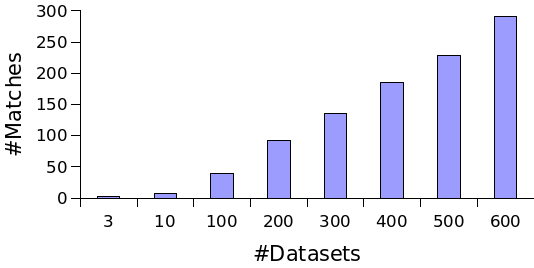
\includegraphics[width=\linewidth]{img/LaundromatDsMatch.png}
	\caption{Dataset Matching (600 datasets LODLaundromat).}
	\label{fig:match600Laundromat}
\end{figure}

The time consumed can be observed on \cref{fig:time600Laundromat}, which shows that 100 million triples were processed in less than 8 minutes, in which is a acceptable time, in which the starts to be time-consuming only after 1 million triples.

\begin{figure}[htb] 
	\centering
	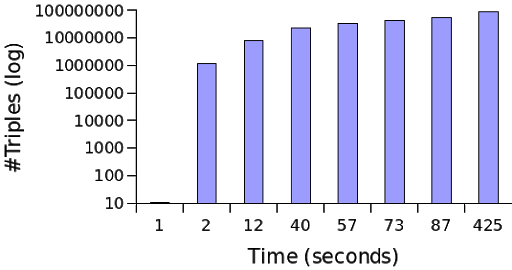
\includegraphics[width=\linewidth]{img/time.png}
	\caption{Time Dataset Matching (600 datasets LODLaundromat).}
	\label{fig:time600Laundromat}
\end{figure}

As we are using WimuQ\cite{valdestilhas2019more} to identify datasets for a given SPARQL query together with our matching algorithm, we can answer the question (2) based on famous Sparql queries from two real-data federated SPARQL querying benchmarks \emph{LargeRDFBench} \cite{largerdfbench2017},\emph{FedBench} \cite{fedbench2011} and one non-federated real data SPARQL benchmark selected from \emph{FEASIBLE} \cite{feasible2015} benchmarks generation framework is given in Figure \ref{fig:numberDatasets1}. Thus, from the selected datasets we use our approach to select the datasets according to the properties and classes they share among them\footnote{In this case, all datasets identified by wimuQ are sharing properties and classes, that is why we are using the graph from \cite{valdestilhas2019more}.}.
% \begin{figure}[htb]
% \centering
%     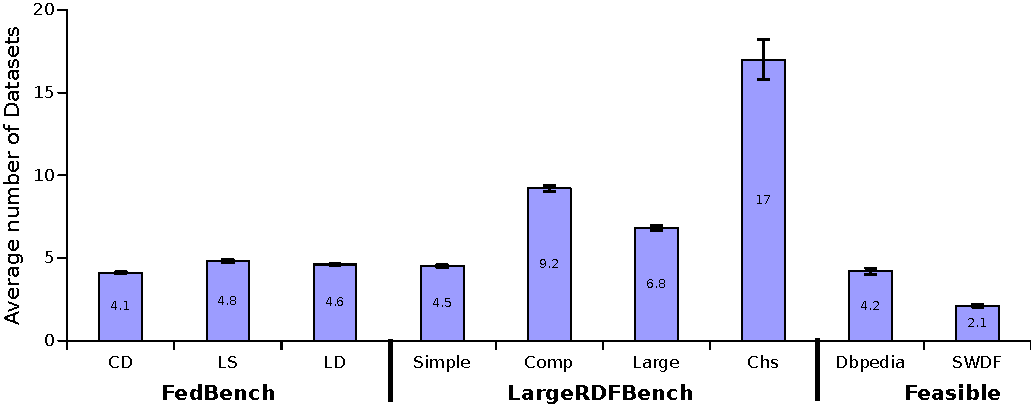
\includegraphics[width=\linewidth]{img/numberDatasets1.pdf}
% 	\caption{Average number of datasets discovered and queried by WimuQ\cite{valdestilhas2019more} across different queries categories of the selected benchmarks.}
% 	\label{fig:numberDatasets1}
% \end{figure}

% To answer the question (3) we have the \cref{fig:md5Namespace} in which we can observe that all datasets from LODLaundromat are named with a MD5 code in which thanks to our approach you can know the domain and namespace information. There are \textbf{X} datasets from LODStats and \textbf{Y} SPARQL endpoints. \todo[inline]{Edgard, please verify and if not created yet, please create a graph/plot/chart fig:md5Namespace containing the info.}

To answer the question (3) we evaluate the dataset duplicated detection algorithm and the detection of dataset chunks.
From a \num{5446} datasets\footnote{A subset from those 600 datasets chosen previously} our algorithm detected \num{2272} duplicates and \num{1470} chunks in 3 hours.

The \cref{fig:identDuplicates} shows a case with 900 datasets chosen randomly, where we identified in 10 cases in which we can see the difference 

The \cref{fig:identChunks} show how many chunks we were able to identify among our sample data, in which lead us to know how segregated is data analysed, giving also the chance to know the complete dataset after the union of all chunks.

\begin{figure}[htb] 
	\centering
	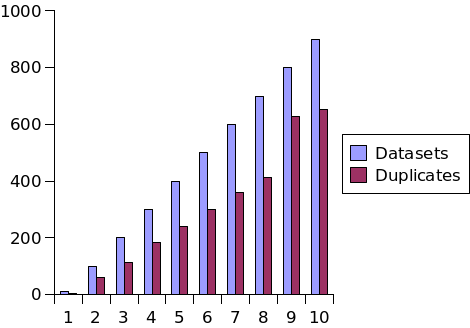
\includegraphics[width=\linewidth]{img/DsDuplicate.png}
	\caption{Duplicates identified in 900 datasets. Y axis represents the number of datasets.}
	\label{fig:identDuplicates}
\end{figure}

\begin{figure}[htb] 
	\centering
	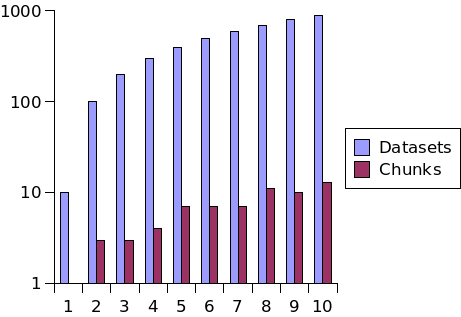
\includegraphics[width=\linewidth]{img/DsChunks.png}
	\caption{Chunks identified in 900 datasets. Y axis represents the number of datasets.}
	\label{fig:identChunks}
\end{figure}

The current version of the index prototype has information about 539 SPARQL endpoints from LOD cloud\footnote{The list of is available here: \url{https://github.com/firmao/wimuT/blob/master/Endpoints_numtriples_lodcloud.csv}} and 915 HDT files from LOD Laundromat\footnote{fdsa}. We perform more than \num{1800000} comparisons in 88 hours.

Where \textbf{DsPropMatch} on the \cref{tab:match} refers to the number of properties/classes the datasets share among each other.

\begin{table}[htb]
    \centering
    \begin{tabular}{|c|c|c|c|c|} \hline
    \textbf{\#Datasets} & \textbf{\#DsPropMatch} & \textbf{time (seconds)} & \textbf{\#triples} & \textbf{Synthetic} \\ \hline
    3 & 2 & 1 & 11 & Yes \\ \hline
    10 & 7 & 2 & 1198508 & no \\ \hline
    100 & 39 & 12 & 7996408 & no \\ \hline
    200 & 92 & 40 & 22982984 & no \\ \hline
    300 & 135 & 57 & 34792121 & no \\ \hline
    400 & 186 & 73 & 43864522 & no \\ \hline
    500 & 229 & 87 & 54227780 & no \\ \hline
    600 & 291 & 425 & 85041239 & no \\ \hline
    \end{tabular}
    \caption{Evaluation on the Match algorithm, where \textbf{DsPropMatch} refers to the number of properties/classes the datasets share among each other.}
    \label{tab:match}
\end{table}

We can observe the quantity of properties/classes that the datasets share related to the number of triples analysed. For instance, from 600 datasets, 291 matches where found, in which the number of triples was almost the double size of the previous case. Thus, the number of matches in this case cannot be directly related to the number of triples. Due to this fact, the quality of the datasets should be considerate a important phase.

We evaluate the accuracy of our matching algorithm with a small sample, where we can see at \cref{fig:fmeasure}, \cref{tab:TableFmeasure} and \cref{fig:runtimeSimilarMatch} the F-Measure and run-time on six famous pairs of datasets from\cite{georgala2018dynamic}, with those datasets we create a gold standard to compare, in which $P_1...P_n$ represents the pair of datasets and P1, P2 are datasets synthetically generated by the author, i.e. P3 represents the comparison between the datasets Abt and Buy.

\begin{figure}[htb] 
	\centering
	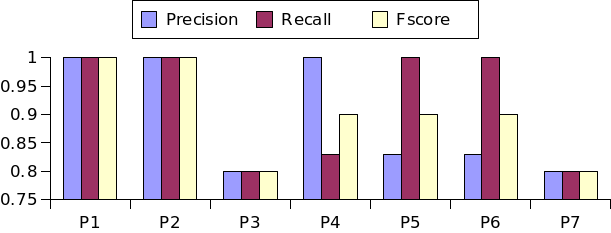
\includegraphics[width=\linewidth]{img/fmeasure.png}
	\caption{F-measure of our string similarity.}
	\label{fig:fmeasure}
\end{figure}

\begin{figure}[htb] 
	\centering
	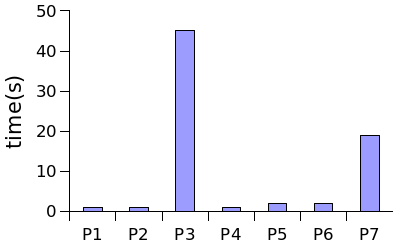
\includegraphics[width=\linewidth]{img/runtime.png}
	\caption{Runtime of our string similarity.}
	\label{fig:runtimeSimilarMatch}
\end{figure}

The \cref{fig:dumps} shows that the majority of files from LODStats are in RDF/XML format.
Moreover, the endpoints are represented in greater numbers (78.6\%), the dominant file format is RDF with 84.1\% of the cases, and 56.2\% of errors occurred because Apache Jena was not able to perform SPARQL queries.
Among the HDT files from LOD Laundromat, 2.3\% of them could not be processed due to parsing errors.
Another relevant point is that 99.2\% of the URIs indexed with WIMU come from LOD Laundromat, due to 69.8\% of datasets from LODstats contain parser errors in which WIMU was not able to process the data.
%https://docs.google.com/spreadsheets/d/15kh8E4WllXG5Xdp1aL-JiHvnXAiVC6a8XqVUJ1gtMZ8/edit?usp=sharing

To answer the question (4) we selected 10 queries\footnote{The queries are available here: \url{https://github.com/firmao/LDatasetGenerator/blob/master/10_Queries_fedbench.txt}} from FedBench\cite{fedbench2011}, where we can observe on the \cref{fig:wimuQRelodDatasets} that thanks to the ReLOD approach we could increase the number of datasets identified by wimuQ, i.e., in query 5, using ReLOD allowed us to find 2 more datasets containing complementary information. 

On the other hand, the \cref{fig:wimuQRelodResults} reinforces that more datasets do not always imply in more results, i.e., in query 2 and 4, more datasets were identified, but the number of results did not change, in this case, the reason was that the datasets identified by ReLOD were practically the same with different property and class names. The results from queries 6 to 10 were only found thanks to the ReLOD approach\footnote{The query number 9 obtained only one result with the new approach.}.

\begin{figure}[htb] 
	\centering
	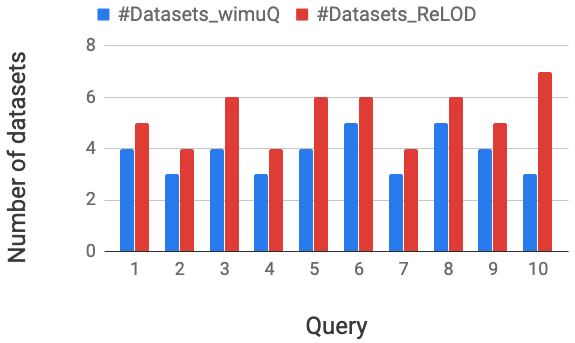
\includegraphics[width=\linewidth]{img/wimuQRelodDatasets.png}
	\caption{Improvement on the number of datasets identified by wimuQ using ReLOD.}
	\label{fig:wimuQRelodDatasets}
\end{figure}

\begin{figure}[htb] 
	\centering
	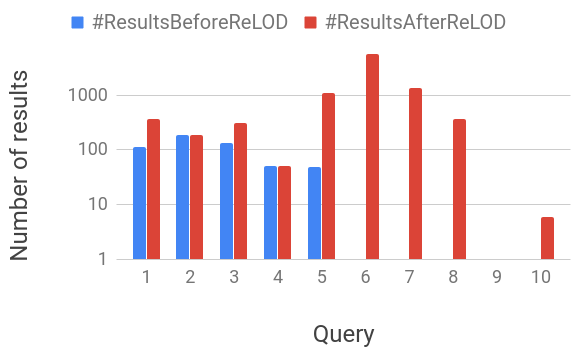
\includegraphics[width=\linewidth]{img/wimuq_relod_results.png}
	\caption{Improvement on the number of results identified by wimuQ using ReLOD. (Vertical axis in log scale).}
	\label{fig:wimuQRelodResults}
\end{figure}

\section{Conclusion}
\label{sec:conc}

With WIMU~\cite{valdestilhas2018my}, we provide a database index of URIs and their respective datasets built upon large Linked Data hubs such as LODStats and LOD Laundromat.
In order to make this data available and easy to use, we developed a semantic web service\footnote{\url{http://wimu.aksw.org/}}.
For a given URI, it is possible to know the dataset the URI likely was defined in using a heuristic based on the number of literals.

With wimuQ\cite{valdestilhas2019more}, we presented an approach to execute SPARQL queries over a large amount of heterogeneous RDF data sources available from different interfaces and in different formats. We made use of the Wimu service to identify the potentially relevant sources to the qiven SPARQL query. We discussed two main types of federated SPARQL query processing approaches namely the endpoints federation and traversal-based federation. The former type of federation only able to execute federated queries over the data available from SPARQL endpoint. While the later, faces problem of URI's dereferenceability. To overcome these issues we proposed a hybrid (endpoints+link-traversal-based) federation engines which integrates four different types of SPARQL query processing engines. Currently, WimuQ\footnote{\url{https://w3id.org/wimuq/}} able to execute both federated and non-federated SPARQL queries over a total of \SI{668}{\kilo\nothing} datasets available from LOD Stats, LOD Laudromat, and LOD cloud active SPARQL endpoints. We evaluated WimuQ by using three state-of-the-art real-data SPARQL benchmarks. We showed that WimuQ is able to successful execute (with some results) majority of the benchmark queries without any prior knowledge of the data sources. In addition, the WimuQ resultset recall is higher with reasonable query execution times. 

With \texttt{ReLOD}\footnote{\url{https://w3id.org/relod}}, we present a method to create a repository to store the similarity between a large number of datasets involving the detection of duplicated datasets and dataset chunks.

The method involves the creation of an index over a total of \num{668166} datasets from LOD Stats and LOD Laundromat as well as 559 active SPARQL endpoints, representing a total of 221.7 billion triples from more than 5 terabytes of information from datasets partially retrieved using the service ``Where is My URI'' (WIMU)\cite{valdestilhas2018my}, in which the query engine wimuQ\cite{valdestilhas2019more} uses the ReLOD to identify the most similar datasets increasing the number of results. 

For the first time, to the best of our knowledge, we make a relation index that can query by dataset URI, property, class, or SPARQL query.

Our experiments show that more than 90\% of datasets from LODLaundromat datasets are not using owl:equivalentProperty and owl:equivalentClass or another way to relate the data, reinforcing the need for an index of relations among LOD datasets.

We realize that the datasets still not sharing the expected properties, and the ontologies are not aligned, making hard the task to query multiple heterogeneous datasets.
We believe that this work can help people to identify similar datasets among a large number of datasets.
As future work, the next step is to improve the GUI drawing a weighted graph that shows the similarity level of each dataset.

We cannot finish this paper without reminding the reader of an aporia in which says - \textit{Different people describe things differently, and this anguish will always lie with us} - That means, at least, this study needs a continuation.

The source-code is available online\footnote{\url{https://github.com/firmao/LODDatasetRelationsWeb}}.

\bibliographystyle{ios1}           % Style BST file.
\bibliography{aksw,ref}        % Bibliography file (usually '*.bib')
\end{document}
